\chapter{方法}

%近年来,随着深度学习在恶意软件检测领域的广泛应用,其高准确率与自动化能力极大提升了防御系统的智能化水平。然而,研究者相继发现深度神经网络存在严重的对抗性脆弱性——即对输入数据中微小扰动高度敏感,这些扰动在肉眼难以察觉的情况下,足以使模型输出完全错误的判断结果。这一特性被攻击者利用,催生出一种新型威胁形式:对抗性恶意软件。

%In recent years, with deep learning widely adopted in malware detection, its high accuracy and automation capabilities have significantly enhanced defense systems’ intelligence. However, researchers have found that deep neural networks exhibit severe adversarial vulnerability, being extremely sensible to subtle disturbances in input data. Imperceptible to humans, these disturbances can cause models to produce entirely incorrect judgments. Attackers utilize this characteristic, catalyzing a novel threat: adversarial malware.

%现有的对抗样本生成方法大多数集中于图像或文本等较为简单的数据类型。然而,在恶意软件领域,尤其是ELF文件等二进制可执行文件,扰动的设计和生成面临更多挑战。恶意软件的结构复杂且精密,任何不当的修改都可能导致文件失效或程序崩溃,因此,如何有效地生成既能绕过检测系统又能够保留恶意功能的对抗样本,是目前面临的核心问题。目前的对抗样本生成技术主要集中在静态和动态扰动上,但依然存在几个关键不足:

%Current adversarial sample generation methods mostly focus on simpler data types like images or text. However, in malware realms, particularly for binary executables like ELF files, disturbance design faces greater challenges. Malware structures are so complex and precise that improper modifications may cause file failure or program crashes. Thus, how to generate adversarial samples that evade detection while ensuring malicious functionalities remains a crucial challenge. Current techniques mainly concentrate on static and dynamic disturbances but still exist critical shortcomings.

\begin{figure}[hbt]
	\centering
	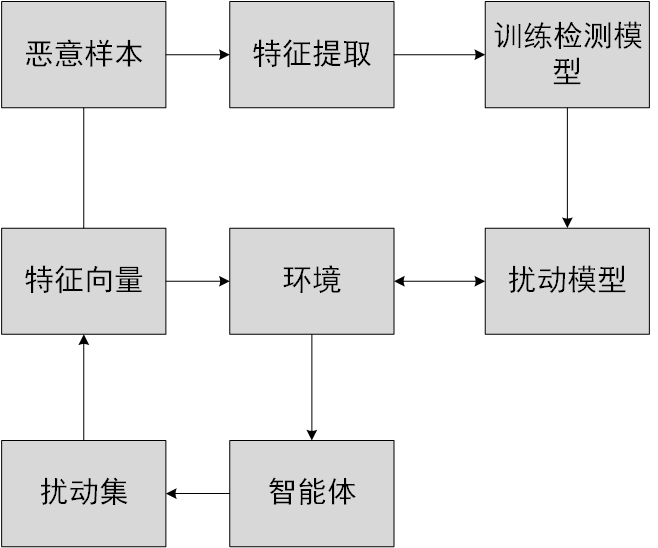
\includegraphics[width=0.75\textwidth]{figures/3.1}
	% \caption[这里的文字将会显示在 listoffigure 中]{这里的文字将会显示在正文中}
	\caption{常见对抗性恶意软件生成模型结构}\label{fig:3.1}
\end{figure}

%\begin{enumerate} [label=\arabic*)] 

%\item 扰动空间的局限性与复杂性

%目前,针对对抗性恶意软件样本的生成,已有方法大多采用如字节插入、修改节区名称、篡改元数据等简单扰动手段来逃避检测系统,这类方法虽然操作便利、实现成本低,但往往缺乏结构感知与语义控制能力,其扰动维度较为单一,不能有效覆盖恶意软件在执行过程中所展现出的复杂特征。在面对复杂结构的二进制文件格式(如ELF)时,盲目扰动极易破坏文件原有逻辑或运行路径,导致样本功能失效或出现运行异常。此外,由于这类扰动方式通常在文件表层留下明显的痕迹,所生成的对抗样本容易被现代静态分析工具或启发式检测系统识别,且对抗效果往往不具备。稳定性和泛化能力。尤其在动态行为检测不断增强的背景下,如何在确保恶意功能完整的同时进行细粒度、多维度、良性扰动,成为当前对抗性样本生成研究中亟待突破的关键问题。

%Existing methods for adversarial malware generation often rely on simplistic disturbances such as byte insertion, section name modification and metadata tampering, to evade detection. Although these methods are convenient to operate and are low cost, they lack structural awareness and semantic control capability. Besides, their disturbance dimensions are insufficient, which makes them hardly cover complex malware features efficiently during execution. For binary files that have intricate structure like ELF, disturbing blindly can easily disrupt file logic or execution paths, causing functional failure or abnormal behavior. Furthermore, such disturbance methods often leave obvious traces on file surfaces, making adversarial samples easily detected by modern static analysis or heuristic systems, which means the adversarial effectiveness lacks stability and generalizability. Especially in the background that dynamic behavioral detection is enhancing continuously, how to perform fine-grained, multi-dimensional and benign disturbances while ensuring functional integrity is a critical challenge to the research.

%\item 扰动的合法性问题

%尽管当前部分对抗样本生成方法在规避恶意软件检测模型方面取得了一定成效,但其扰动策略普遍存在粗糙和随机性强的问题,常见手段包括随机字节插入、伪装节名称、修改冗余字段等浅层扰动。这类方法虽能在某些静态检测模型中绕过特征匹配机制,但缺乏对扰动合法性与语义一致性的有效控制,难以适应真实环境下多样化且复杂的检测机制。例如,随意插入的字节可能被高级检测模型识别为异常行为(如零号攻击),反而增强了恶意特征的可识别性。尤其对于依赖行为分析或异常检测的模型而言,盲目的扰动不仅无助于逃避检测,反而可能使模型学习到更具代表性的恶意特征,从而降低对抗攻击的有效性。此类“为扰动而扰动”的生成策略虽然可能在静态条件下取得短期成功,但难以保障在实际部署环境中的稳定性与隐蔽性。因此,如何构建更加结构化、具备语义感知能力的扰动策略,在不破坏原有功能的前提下提升扰动的针对性与有效性,成为当前对抗性恶意样本生成研究中的关键挑战之一。

%Although current adversarial generation methods succeed in evading malware detection models, their disturbance strategies tend to be crude and highly random. Common operations include surface-level disturbances such as random byte insertion, disguised section names, and redundant byte modification. While features evade matching in static detectors, they lack effective control over disturbances legitimacy and semantic consistency, struggling against diverse real environments and detection mechanisms. For example, bytes inserted randomly may be recognized as abnormal behaviors such as zero-day attacks by advanced models, enhancing malicious feature detectability. Particularly for detection models based on behavior analysis or abnormal behavior detection, blind disturbances not only fail to evade detection but also risk teaching models more representative malicious features, reducing attack efficiency. Such strategies whose activities are only to disturb without considering effectiveness may achieve short-term static evasion but lack stability and concealment in a real deployment environment. Therefore, developing strategies that are more structural, high awareness to semantic to enhance precision and validity without losing origin functionalities is crucial.

%\item 对历史扰动的依赖性缺失

%对抗样本的生成过程本质上是一个动态决策序列,其扰动操作并非孤立发生,而是具有明显的时序依赖性——当前的扰动决策往往会受到先前扰动历史的影响。然而,现有的主流对抗样本生成方法大多将每一步扰动视为独立事件,缺乏对扰动序列内在依赖关系的建模与挖掘。这种近似于“无记忆”的策略忽略了扰动间的逻辑联系与语义上下文,导致生成的扰动序列在结构上缺乏连贯性,扰动操作之间相互脱节,甚至可能出现前后矛盾或重复无效的修改操作。这不仅降低了对抗样本的逃避能力和隐蔽性,还可能引入可疑的行为模式,反而提升被检测的风险。特别是在处理结构复杂、语义敏感的二进制恶意样本时,忽视扰动间依赖会进一步削弱攻击效果。因此,如何引入有效的时序建模机制,捕捉扰动操作之间的动态关联,从而生成更具整体性、策略性和欺骗性的扰动序列,是提升对抗样本实战能力的关键突破方向之一。

%Adversarial sample generation is a dynamic decision-making sequence. Disturbance operations manifest sequential dependencies: current decisions depend on prior perturbation history, instead of isolation. However, prevalent methods treat each disturbance step as isolated, neglecting to find the inherent dependency relations. This approximately memoryless strategy ignores logical and semantic contexts between disturbances, resulting in generated sequences structural succession deficiency and disturbance operations disconnected from each other, which exhibits that some modification operations contradict with previous operations or duplicated. This result not only undermines adversarial samples’ evasion capabilities and concealment, but also potentially introduces suspicious action patterns that increase the detected rate. Especially in structurally complex, semantically sensitive malware binaries, overlooking the dependence between disturbances further reduces attack effectiveness. Therefore, introducing effective temporal modeling mechanisms to capture dynamic correlations in disturbance operations and generating more integral, strategic, deceptive disturbance sequences is a key breakthrough in enhancing adversarial sample capacities in real environments.

%\item 过于关注逃逸率,忽视扰动成本与执行开销 

%当前许多对抗性恶意软件生成方法普遍将“是否成功逃逸检测系统”作为主要评价指标,过度聚焦于误分类结果,而忽略了扰动过程中的多方面代价。在实际应用中,生成的对抗样本不仅需要具备较强的逃逸能力,还应兼顾扰动的实施成本与执行效率。例如,频繁或复杂的扰动操作可能导致样本体积显著增加、运行时间延长,甚至影响程序的原有功能和行为一致性,从而在实际环境中暴露风险。此外,部分策略在扰动选择上未考虑操作本身的资源消耗和可行性,导致生成的样本难以在有限计算资源下快速部署。忽视这些现实因素,往往使得对抗样本虽然能在检测模型层面绕过检查,但却在工程实际中难以落地。因此,仅以逃逸率为单一优化目标的生成策略存在明显局限,亟需引入对扰动成本与时间开销的系统性考量,以提升对抗样本的实用性与隐蔽性。

%Many current adversarial malware methods mostly regard "successfully evading malware detection systems" as the primary evaluation metric, overemphasizing misclassification results while ignoring multifaceted costs of disturbance processes. However, in practical applications, not only high evasion capacities are required to adversarial samples generated, but also keeping the balance of implementation costs and execution efficiency. For example, excessive or complex disturbances significantly increase file size, prolong runtime, disrupt functionality, or affect behavioral consistency, which potentially exposes risks during execution. Furthermore, some strategies overlook resource consumption and feasibility of operations, rendering generated samples hard to deploy under constrained resources. Although ignoring these real-world factors allows samples to bypass detection models, it is a failure in engineering deployment. Therefore, the strategy that regards evasion rate as the only optimization exhibits significant limitations. It is urgent to introduce systemic consideration of disturbance costs and time to enhance sample practicality and concealment.

%\end{enumerate}

%本文主要的研究目的是借助强化学习和神经网络方法,构建多维度和高效的对抗样本生成方法。针对目前已有研究方法中存在的不足,本文提出以下需要解决的关键问题:

%The primary objective of this research is to construct a multidimensional and efficient adversarial sample generation approach utilizing reinforcement learning and neural network methods. Addressing the shortcomings of existing methods, the following critical issues are required to resolve:

%关键问题1:如何构建一个具备结构感知和语义控制能力的多维度扰动空间,以适应复杂恶意软件样本的逃逸需求?

%Key Issue 1: How to construct a multidimensional disturbance space with structural awareness and semantic control capability to meet the evasion needs of complex malware samples?

%关键问题2:如何提升扰动的合法性与良性,避免传统“破坏式扰动”在真实检测系统中反而暴露攻击意图?

%Key Issue 2: How to enhance disturbance legitimacy and benignity, avoiding traditional "destructive disturbances" that may expose attack intentions in real detection systems?

%关键问题3:如何引入扰动历史建模机制,从而生成更具连贯性和策略性的扰动序列?

%Key Issue 3: How to introduce historical disturbance modeling mechanisms to generate more coherent and strategic disturbance sequences?

%关键问题4:如何在对抗样本生成过程中权衡扰动有效性、功能完整性与资源开销,提升攻击样本的实际可部署性?

%Key Issue 4: How to balance effectiveness, functional integrity, and resource consumption during adversarial sample generation to enhance the practical deployability of attack samples?

\section{方法概述}
针对当前对抗性恶意软件样本生成方法在扰动手段粗糙、语义控制能力弱、扰动序列缺乏结构性以及忽视现实成本与可部署性等方面的不足,本文提出了一种创新的对抗样本生成框架。现有方法通常依赖简单且随机的字节插入、修改节名称等手段,缺乏对生成样本的合法性、语义一致性以及可执行性的有效控制,导致在实际环境中难以稳定有效地逃避检测。因此,本文的研究思路旨在通过系统性地优化对抗样本生成的多个关键方面,弥补这些不足。

%To address current adversarial malware generation methods' limitations in coarse perturbation techniques, weak semantic control, lack of structural disturbance sequences, and neglect of practical costs and deployability, this research proposes an innovative adversarial sample generation framework. Common existing methods rely on simple, random byte insertions or section name modifications that lack effective control over sample legitimacy, semantic consistency, and executability, resulting in unstable evasion in real environments. Therefore, this research aims to solve these shortcomings by systematically optimizing multiple key aspects of adversarial sample generation.

首先,在扰动空间建模方面,本文通过引入多维度扰动技术,打破了传统方法只依赖单一扰动手段的局限,考虑到恶意软件在不同执行阶段可能展现出的多样化特征,设计了一种结构化且具有语义感知能力的扰动策略,从而避免了对文件功能的破坏,同时提高了逃避检测的难度。其次,针对扰动合法性问题,本文提出了一种基于语义一致性的扰动合法性控制方法,确保生成的对抗样本在避开检测的同时,能够维持原有的功能和行为一致性,避免了盲目扰动所带来的不稳定性。

%Firstly, in the disturbance space modeling aspect, this paper introduces multidimensional disturbance techniques and breaks the limitation of traditional methods that solely rely on single disturbance methods. Since malware exhibits diverse features in different execution stages, this research designs a structural disturbance strategy with semantic awareness capacities, avoiding file functionality disruption and enhancing evasion difficulties. Secondly, targeting the disturbance legitimacy issue, a disturbance legitimacy control method based on semantic consistency is proposed to ensure adversarial samples evade detection while maintaining original functionality and behavioral consistency, avoiding instability from blind disturbances.

另外,考虑到对抗样本生成过程中的扰动序列具有明显的时序依赖性,本文通过强化学习中的PPO算法结合LSTM网络对扰动序列进行建模,从而有效捕捉扰动操作之间的动态关系,使得生成的扰动序列在整体上更加连贯、隐蔽和具备欺骗性。通过这一方法,能够优化扰动的执行顺序和策略,进一步提升对抗样本的逃避能力。

%Furthermore, recognizing the obvious temporal dependency in disturbance sequences, this research employs the PPO algorithm combined with LSTM networks to model disturbance sequences, effectively capturing dynamic relationships between disturbances. This approach enhances the overall coherence, stealth, and deceptive nature of disturbance sequences, optimizing the order and strategies to further improve evasion capabilities.

最后,针对现有方法忽视扰动过程中的成本与可执行性问题,本文提出了一种新的奖励机制,除了关注检测逃逸率外,还考虑了生成过程中的资源消耗、执行时间等因素,确保生成的对抗样本不仅具备较高的攻击性,还能够在实际环境中顺利部署,避免因过于复杂的扰动操作导致样本体积膨胀、运行时间延长或功能丧失。

%Lastly, addressing the neglect of disturbance costs and executability, a new reward mechanism is proposed in this research. Except for focusing on evasion rates, it considers different factors such as resource consumption and execution time, ensuring that adversarial samples are not only highly aggressive but also deployable in real environments. This prevents sample size surges, prolonged runtime, or functional loss caused by excessive disturbances.

%与传统方法相比,本文具有以下几个显著优点:

%\begin{enumerate} [label=\arabic*)] 

%\item 结构感知的扰动空间构建:突破以往依赖静态规则或单一字节操作的扰动方式,本文在样本的结构层与语义层中引入更细粒度的操作集,设计出支持多维度、多粒度扰动的操作空间,能够更精准地定位关键行为区域并施加微扰动,从而有效提升逃避检测的灵活性和有效性。

%Structurally Aware Perturbation Space Construction: Departing from previous disturbance methods relying on static rules or single-byte operations, this research introduces a finer-grained operation set at the structural and semantic layers of samples, designing an operational space supporting multidimensional and multigranular disturbances, enabling to localize key behavioral regions more precisely and apply subtle disturbances, thereby effectively enhancing the flexibility and effectiveness of evasion detection.

%\item 扰动合法性与语义一致性的融合控制机制:不同于以往“只求误判、不管后果”的扰动逻辑,本文在生成过程中引入语义保持约束与合法性验证策略,确保扰动不会破坏程序原有逻辑与可执行性,从而提升对抗样本在真实系统中的稳定性与隐蔽性。

%Fusion Control Mechanism for Disturbance Legitimacy and Semantic Consistency: Unlike the previous disturbance logic that only pursues misclassification regardless of consequences, this research incorporates semantic preservation constraints and legitimacy verification strategies during the generation process, which ensures that disturbances do not disrupt the original program logic and executability, enhancing the stability and concealment of adversarial samples in real systems.

%\item 考虑扰动历史的序列建模机制:本文将对抗扰动过程视为一个具有时序依赖特征的策略优化任务,引入序列建模机制(如记忆单元或策略网络)来捕捉扰动操作之间的上下文关系,使生成的扰动序列更具策略性与一致性,解决了以往扰动碎片化、冗余化的问题。

%Sequence Modeling Mechanism Considering Disturbance History: This research regards the adversarial disturbance process as a strategy optimization task that exhibits temporal dependency characteristics. It introduces sequence modeling mechanisms, such as memory cells or policy networks, to capture the contextual relationships between disturbance operations, which enables the sequences generated to be more strategic and consistent, addressing the previous issues that disturbances are fragmented and redundant.

%\item 面向成本与开销的实用性优化目标:本文在对抗目标设计中充分考虑扰动的实施成本、样本运行效率和部署风险等实际因素,引入“轻量扰动”与“开销评估”机制,有效控制扰动规模和复杂度,使生成样本更具工程实用性,避免“虽逃逸成功却难以部署”的局限。

%Optimization Objective Oriented towards Cost and Overhead Practicality: In designing the adversarial objectives, this research fully considers practical factors such as disturbance implementation cost, sample runtime efficiency, and deployment risk, introducing "lightweight perturbation" and "overhead assessment" mechanisms to effectively control the scale and complexity of disturbances. This makes the samples generated more practical for engineering deployment, thus avoiding the limitation of being evasive but hard to deploy.

%\end{enumerate}

%\section{研究的解决方案 Research Solutions}

%针对本文3.1节中当前对抗性恶意软件样本生成方法中存在的扰动手段粗糙、语义控制能力弱、扰动序列缺乏结构性以及忽视现实成本与可部署性等问题,本文提出了一种面向实用性与隐蔽性强化的对抗样本生成框架。该框架从多个维度出发,提出了四个关键解决方案,以提高对抗样本的生成能力、逃避检测效果及实用性。

%To address the issues in Section 3.1—that disturbance methods are coarse, weak semantic control, lack of structural disturbance sequences, and neglect practical costs and deployability—this paper proposes a novel adversarial sample generation framework facing practicality and concealment enhancement. This framework focuses on enhancing generation capabilities, evasion effectiveness, and practicality through 4 key solutions.

%解决方案1:基于多维度的扰动空间建模

%Solution 1: Disturbance Space Modeling Based on Multi-dimensions

%传统的对抗样本生成方法通常采用简单的扰动方式,如字节插入、节区名称修改、冗余字段篡改等,这些方法虽然在短期内能够绕过检测,但其扰动空间较为有限,无法有效应对恶意软件复杂执行过程中的多样化特征。为此,本文提出了一种多维度扰动策略,通过精确建模多种扰动维度,从结构、指令、行为三个层面对扰动空间建模以全面覆盖恶意软件在执行过程中可能展现出的行为特征。该策略能够有效提高恶意软件样本的逃避能力和隐蔽性,同时保持样本的功能完整性。在扰动设计中,特别关注对恶意代码执行路径、控制流及其他关键结构的精确干扰,从而最大程度避免传统方法中存在的结构损坏和功能失效的问题。

%Traditional adversarial sample generation methods usually employ simple disturbances, such as byte insertion, section name modification, or redundant byte modifications. While these methods may temporarily evade detection, their disturbance space is limited, failing to address the diverse features exhibited during malware execution. To address this issue, this paper proposes a multidimensional perturbation strategy. By precisely modeling various disturbance dimensions, this approach constructs a disturbance space across structural, instruction, and behavioral layers, comprehensively covering potential behavioral features during malware execution. This strategy enhances the evasion and concealment capabilities of malicious samples while preserving their functional integrity. Disturbance design particularly targets precise interference with malicious code execution paths, control flows, and other critical structures, minimizing structural damage and functional failure issues in traditional methods.

%解决方案2:基于良性样本的合理化插入扰动

%Solution 2: Rationalized Insertion Disturbance Based on Benign Samples

%当前许多对抗样本生成方法的扰动通常依赖于随机字节插入等浅层操作,这种方式缺乏对语义合法性和扰动合理性的控制,容易导致生成样本的不稳定性或被检测到。为了解决这一问题,本文提出了一种基于良性样本的合理插入扰动方法。在这一方法中,首先通过分析良性样本的结构与行为,提取出良性样本的语义与字节结构,构建良性样本扰动库。通过对扰动进行更加结构化和语义感知的设计,保证了对抗样本在功能上的完整性和合法性,同时减少了不必要的噪声扰动。这种方法不仅能有效规避基于特征匹配的静态检测系统,还能增强对抗样本在复杂检测环境中的隐蔽性。

%Current adversarial sample generation methods often rely on shallow operations, such as random byte insertion, lacking control over semantic legitimacy and disturbance rationality. This can lead samples to be unstable and to be detected easily. To overcome this disadvantage, this paper introduces a rationalized insertion disturbance method based on benign samples. By analyzing the structure and behavior of benign samples, their semantic and byte structure are extracted to build a benign sample perturbation library. This method ensures functional completeness and legitimacy of adversarial samples through more structurally and semantically aware disturbance design, reducing unnecessary noise. It not only effectively evades static detection systems based on feature matching but also enhances sample concealment in complex detection environments.

%解决方案3:基于LSTM的PPO时序依赖建模

%Solution 3: PPO Temporal Dependency Modeling Based on LSTM

%对抗样本的生成不仅仅是每一步独立的扰动操作,而是一个具有时序依赖性的过程。现有方法通常忽略了扰动间的依赖关系,导致生成的扰动序列缺乏整体性和连贯性,从而影响逃避能力。为了解决这一问题,本文结合PPO\cite{yu2022surprising}(Proximal Policy Optimization)强化学习算法和LSTM\cite{graves2012long}(Long Short-Term Memory)模型,提出了一个联合优化的时序依赖建模方法。通过LSTM网络对扰动序列的时序关系进行建模,捕捉扰动之间的内在依赖性,PPO算法则用于优化生成策略。这一方法能够生成更具整体性、连贯性和隐蔽性的扰动序列,有效提升对抗样本的攻击性和稳定性。

%Adversarial sample generation is not merely a series of independent disturbances but a process with temporal dependencies. Existing methods often overlook dependencies among different disturbances, resulting in disjointed sequences and reduced evasion capabilities. To solve this issue, this paper combines the PPO Reinforcement Learning algorithm\cite{yu2022surprising} with LSTM\cite{graves2012long} models to propose a joint optimization method for temporal dependency modeling. LSTM networks model temporal relationships in disturbance sequences, capturing intrinsic dependencies among disturbance operations, while PPO optimizes generation strategies. This method produces holistic, coherent, and stealthy disturbance sequences, enhancing adversarial sample attack effectiveness and stability.

%解决方案4:基于动态奖励函数的智能体决策

%Solution 4: Decision-Making Agent Based on Dynamic Reward Functions

%在现有的对抗样本生成方法中,奖励函数设计往往过于简单,通常只关注样本是否成功绕过检测系统,而忽略了生成过程中的成本与效率问题。为了克服这一不足,本文提出了一种基于动态奖励函数的智能体决策机制。该机制不仅考虑逃逸成功与误分类率,还引入了扰动的资源消耗、执行效率、时间开销等因素。通过这种动态奖励机制,智能体在决策过程中能够更好地平衡攻击性与执行代价,从而生成既具备高隐蔽性,又能够快速部署的对抗样本。该方法有效提升了对抗样本的实际应用价值和部署可行性。

%Existing adversarial sample generation methods often employ simplistic reward functions focused solely on whether the sample evades the detection systems, neglecting generation costs and efficiency. To address this disadvantage, this research proposes an agent-making mechanism based on dynamic reward functions. Beyond considering evasion success and misclassification rates, it incorporates factors, such as disturbance resource consumption, execution efficiency, and time costs. This dynamic reward mechanism enables agents to balance attack effectiveness with execution costs during decision-making, generating adversarial samples that are both highly stealthy and quickly deployable. This approach significantly enhances the practical application value and deployability of adversarial samples.

\section{数据收集与预处理}

%为了有效应对恶意软件检测系统的不断演进,提升对抗样本在真实环境下的生存能力与攻击效果,本文提出了一套系统化的对抗样本生成架构。整体设计遵循分层递进、策略引导、效果评估的原则,涵盖了数据收集、扰动策略建模、强化学习智能体训练以及奖励函数设计等关键环节,确保对抗样本能够在保证功能正确性的前提下,最大程度逃逸各类检测系统的拦截。

%To effectively address evolving malware detection systems and enhance the survivability and attack effectiveness of adversarial samples in real environments, this research proposes a systematic adversarial sample generation framework.Its overall design follows principles of hierarchical progression, strategy guidance, and effect evaluation and contains key components, such as data collection, disturbance strategy modeling, RL agent training, and reward function design, ensuring adversarial samples maximize evasion rate across various detection systems while maintaining functional correctness.

%\begin{enumerate} [label=(\arabic*)] 



%(1) Data Collection and Preprocessing

高质量的数据基础是对抗样本生成系统有效运行的关键前提,尤其是在针对ELF格式可执行文件的研究中,由于当前尚缺乏权威性、标准化的公开数据集,这一问题尤为突出。为弥补该空白,本文自主构建了一个覆盖面广、结构多样的ELF样本集,涵盖恶意样本与正常样本两个维度,确保后续模型训练与扰动策略评估具有良好的实验基础与推广能力。

%High-quality data is fundamental to the adversarial sample generation system effective operation, especially dominant for ELF-format executable file research due to the current lack of authoritative, standardized public datasets. To bridge this gap, this research constructs a full-coverage, structurally diverse ELF sample set, including both malicious and benign samples, ensuring a robust experimental foundation and promotion capability for model training and disturbance strategy evaluation.

在恶意样本采集方面,本文主要从VirusShare\cite{VirusShare}、Maltrieve等知名的开源恶意软件平台中筛选并下载经过多重验证的x86架构下的ELF格式恶意样本。样本类型涵盖多种常见攻击形式,包括蠕虫传播程序、加密货币挖矿程序、远程控制型后门程序、DDoS工具及嵌入式木马等,具有较强的代表性与研究价值。为进一步提升样本质量,本文对收集到的样本进行了格式校验、哈希去重、恶意行为标签确认等预处理操作,确保样本集的真实性与一致性。在正常样本采集方面,本文基于QEMU虚拟化技术搭建了多个目标运行环境,主要包括基于Raspbian和OpenWrt的ARM架构嵌入式系统,以及基于Ubuntu的x86系统环境,从中提取了系统默认运行的合法ELF程序,如系统工具、守护进程、配置脚本等。这些样本在功能完备、结构规范的同时,能够覆盖多种开发工具链和构建方式,进一步增强了正常样本集的多样性与代表性。

%For malicious sample collection in this research, verified ELF-format malware samples targeting x86 architecture were sifted and downloaded from renowned open-source platforms such as VirusShare\cite{VirusShare} and Maltrieve. These samples cover common attack types, such as worm propagation programs, cryptocurrency miners, remote-controlled backdoors, DDoS tools, and embedded Trojans, offering strong representativeness and research value. To enhance sample quality, format validation, duplicate hash removal, and malicious behavior label verification were performed to ensure authenticity and consistency.For benign sample collection in this research, multiple target runtime environments were established using QEMU virtualization technology, including ARM-based embedded systems like Raspbian and OpenWrt, and x86-based systems like Ubuntu. Legitimate ELF programs, such as system tools, daemons, and configuration scripts were extracted from those embedded systems. These samples, being functionally complete and structurally standard, cover various development tool chains and build methods, enhancing the diversity and representativeness of the benign sample set.

为了确保数据集的质量与准确性,本文在完成初步样本收集后,针对所有获取的ELF格式可执行文件样本均引入了VirusTotal\cite{VirusTotal}平台的复审机制,以增强样本标注的权威性与恶意性确认的可信度。具体而言,首先对每个样本执行SHA-256等哈希指纹提取操作,构建唯一标识,剔除重复或冗余的样本项,确保样本集的去重和纯净;随后将样本上传至VirusTotal平台,通过其集成的多引擎病毒扫描系统(涵盖Kaspersky、Avast、BitDefender、ESET等多个主流安全厂商)进行全面检测。

%To ensure dataset quality and accuracy, after initial sample collection, a review mechanism from the VirusTotal\cite{VirusTotal} platform was introduced for all collected ELF executable samples, strengthening the authority of label notes annotation and the credibility of maliciousness confirmation. In detail, first, hash fingerprints like SHA-256 are extracted from each sample to create unique identifiers, removing duplicate and redundant samples. Second, samples are uploaded to VirusTotal for comprehensive detection by using integrated multiple engines that contain Kaspersky, Avast, BitDefender, and ESET. 

在扫描过程中,本文重点关注引擎返回的检测标签、恶意评分(malicious score)、行为分析结果以及YARA规则匹配情况等关键信息,构建每个样本对应的检测报告元数据集,用于后续的分析、训练与评估。同时,对于存在标注不一致或引擎分歧较大的边界样本,通过引入手动复审或多轮投票方式进一步判断其可信分类,保证数据标注的一致性和准确性。
此外,扫描报告中所提取的信息(如API调用特征、连接行为、时间戳等)也为后续的扰动操作设计与对抗样本生成提供了参考依据,帮助理解当前主流检测机制所侧重的关键特征,从而指导扰动策略选择。

%In the scanning process, this research concentrates on critical information, including detection tags, malicious scores, behavioral analysis results and YARA rule matches returned by engines, which are used to construct a metadata report for each sample for subsequent analysis, training and evaluation. Besides, manual review and multi-round voting are introduced to judge and classify marginal samples that exhibit annotation inconsistency or significant engine disagreements, ensuring data annotation consistency and accuracy. Furthermore, information extracted from the scan reports, such as API call signatures, connection behaviors, and timestamps, also serves as a reference for subsequent disturbance design and adversarial sample generation, helping to identify key features prioritized by current detection mechanisms and guiding disturbance strategy selection.


\section{扰动策略构建}

%(2) Disturbance Strategy Construction

针对现代恶意软件检测系统在静态、动态以及行为特征等多维度的集成分析机制,本文提出了一种具有分层次特征的组合式扰动策略,旨在从结构信息、指令序列和动态行为三个层面入手,打破传统特征提取链条,从而提升对抗样本的隐蔽性与鲁棒性。在现有检测系统中,往往通过固定规则或训练模型提取静态特征(如节结构、函数调用图、符号信息)、指令级特征(如n-gram、CFG路径)以及动态行为(如系统调用序列、内存行为等),因此,设计能够有效扰乱这些检测路径的扰动机制对于生成高质量对抗样本具有重要意义。

%To counter modern malware detection systems' integrated analysis across static, dynamic, and behavioral features, this research proposes a hierarchical combined disturbance strategy that targets to disrupt traditional feature extraction chains through three levels—structural information, instruction sequences, and dynamic behaviors, enhancing the concealment and robustness of adversarial samples. Since current detection systems typically rely on fixed rules or trained models to extract static features, such as section structures, function call graphs, symbol info, instruction-level features, such as n-grams and CFG paths, and dynamic behaviors such as system call sequences, memory behaviors, thus, designing disturbance mechanisms effective against these detection paths is crucial for generating high-quality adversarial samples.

在结构扰动方面,本文主要采用插入式结构变换策略,该策略具有较好的通用性和对原程序功能的非破坏性。具体方法包括在ELF二进制文件中插入伪造节(section)和无效段(segment),例如通过LIEF库\cite{LIEF2025}动态创建.fake、.dummy\_code等节,且这些节不参与程序逻辑流程,仅作为混淆成分存在;同时对ELF头部(ELF Header)、程序头表(Program Header Table)及节区头表(Section Header Table)进行轻量修改,如调整节表顺序、伪造入口点地址、添加重定位信息等,使得静态分析工具在解析时产生偏差。此外,还包括对程序进行壳处理(packing)和脱壳(unpacking)操作,通过UPX等压缩工具实现结构扰动,并结合反壳策略恢复执行能力,从而扰乱基于字节签名和结构模式匹配的检测系统。

%In structural disturbance aspect, this research mainly adopts structural transformation strategies based on insertion that exhibit high adaptivity and are not disruptive to original program functionalities. Concrete methods include inserting fake sections and invalid segments in ELF binary files, such as dynamically create sections that are only used for obfuscation and do not engage program logic processes, such as .fake and .dummy\_code, by using LIEF \cite{LIEF2025} library. Additionally, slight ELF Header, Program Header Table and Section Header Table adjustments, including altering section table sequences, fabricating the entry point address and adding relocation information, induce parsing errors in static analysis tools. Furthermore, packing and unpacking structural disturbance operations via compression tools like UPX, along with strategies to restore execution capability, confuse detection systems based on byte signature and structural pattern comparison. 

\begin{figure}[hbt]
	\centering
	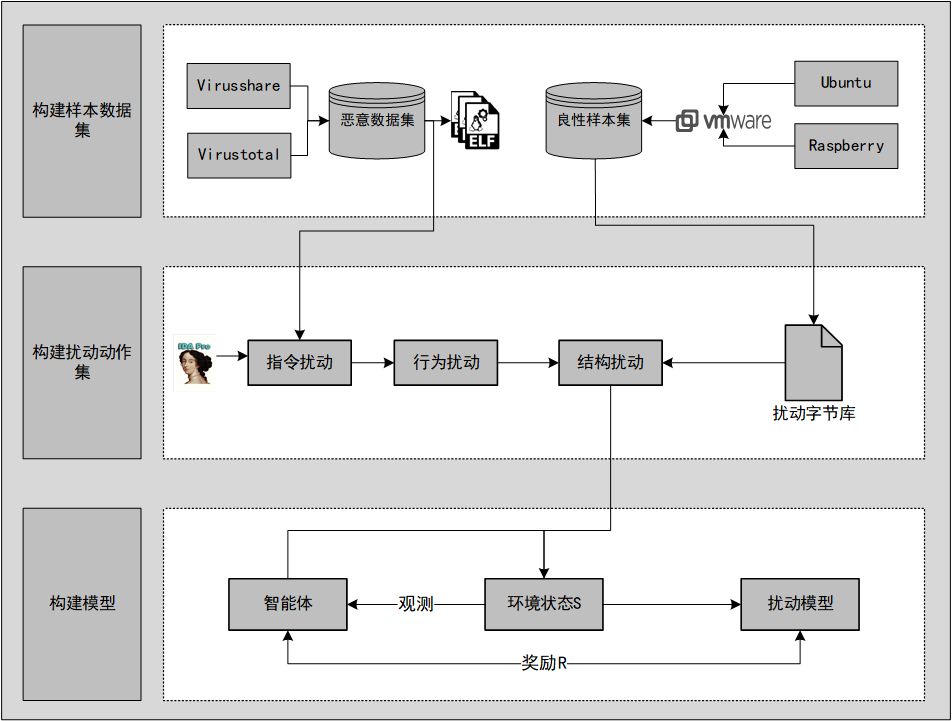
\includegraphics[width=0.75\textwidth]{figures/3.2}
	% \caption[这里的文字将会显示在 listoffigure 中]{这里的文字将会显示在正文中}
	\caption{基于强化学习的对抗性样本生成方法框架}\label{fig:3.2}
\end{figure}


在指令层面,本文通过结合IDA Pro、radare2等反汇编工具,对原始二进制样本进行静态反汇编与控制流图提取,进而实现对指令的扰动式重写。首先,在保证程序语义不变的前提下,使用等价指令替换技术,例如用xor eax, eax替换mov eax, 0,或使用冗余的加法/减法指令链完成简单赋值,扰乱检测模型对常规语义的理解;其次,利用寄存器交换策略(如将eax换为ebx等)打破寄存器使用模式,同时修改跳转指令逻辑,在跳转目标不变的情况下引入间接跳转、中间跳板、无效跳转等手段,以此增加CFG的复杂度,干扰以控制流为特征的静态图分析器。在指令组合上,本文还引入了无效填充操作,如NOP滑块(NOP sled)与空函数调用序列,进一步加大模型提取有效语义片段的难度。

%In the instruction layer, this research used disassembly tools, such as IDA Pro and radare2, to disassemble original binary samples and extract control flow graphs to achieve instruction disturbance. First, in the background that program semantics are not disrupted, equivalent instruction replacements, such as using “xor eax, eax” to replace “mov eax, 0” and using redundant arithmetic chains to achieve simple assignments, disturb common semantic understanding for detection models. Second, utilizing register swapping strategies like replacing “eax” with “ebx” changes register usage patterns and modifies instruction jump logic. Indirect jumps and invalid jumps are introduced to increase CFG complexity to disturb static diagram analyzer targeted on CFG features with the premise that jump target is not changed. In the instruction combination realm, this research introduces invalid padding operations, such as NOP sled and empty function call sequences, to increase the difficulty of extracting meaningful semantic segments.

针对动态分析系统的行为建模特性,本文设计了一套动态执行扰动机制,旨在规避基于沙箱技术的行为检测模型。该机制通过修改程序实际入口点(Entry Point),优先执行伪造行为逻辑,再逐步过渡到真实恶意载荷执行,从而在短时间行为采集窗口中有效延迟真实行为暴露。常用策略包括添加自循环逻辑(例如构造伪循环结构)、空跳转路径(无逻辑变化但执行时间延长)以及插入系统级延迟调用,如sleep()、nanosleep()等API,来阻断沙箱的行为提取流程。此外,还可嵌入虚拟环境检测语句(如CPUID指令、MAC地址识别等),使得样本在虚拟分析平台上呈现不同行为路径,进一步规避检测。结合动态段的无效控制流插入,本文的扰动策略在沙箱动态行为分析阶段展现出良好的逃避性能。

%To address dynamic analysis system behavioral model features, this research design a dynamic execution disturbance mechanism aims to evade behavioral detection models based on sandbox techniques. This mechanism modifies the actual Entry Point, prioritizes executing fabricated behavioral logic and then gradually executes true malicious code, effectively postponing the exposure of factual behaviors in windows that capture behaviors. Common strategies include self-loop logic, such as fabricated loop structures, empty jump paths that do not affect program execution logic but prolong execution time and delayed APIs insertions, such as sleep() and nanosleep(), which prevent sandbox extraction workflows. Furthermore, virtual environment detection functions, such as CPUID instructions and MAC address identification instructions, can also be embedded to make samples exhibit different behaviors on platform based on virtual analysis. Combined with inserting invalid control flows into dynamic segments, these disturbance strategies demonstrate strong evasion capabilities during dynamic behavior analysis based on sandboxes.

\subsection{结构化扰动方法}

在恶意软件的对抗性样本生成过程中,结构层面的扰动指的是通过修改文件的内部结构来引入变化,这种变化通常不会影响文件的执行逻辑,但能够有效地逃避传统的检测方法。结构层面的扰动包括但不限于文件的节区、导入符号、动态库、以及压缩/解压缩等操作。

%In the adversarial malware sample generation process, structural level disturbances refer to introducing changes by modifying a file's internal structure. These changes commonly do not affect the file's execution logic but effectively evade traditional detection methods. Structural level disturbances include operations on sections, imported symbols, dynamic libraries, compression, and decompression, but are not limited to these.

这些扰动主要关注的是通过改变文件结构中的某些元素来达到以下目的:
%These disturbances primarily concentrate on achieving the following purposes by altering certain elements in the file structure:
\begin{enumerate}
	 
\item 增加文件的不可预测性:通过随机化或改变文件的某些部分,使得检测系统很难依赖固定模式进行识别。
%Increasing file unpredictability: By randomizing or changing parts of the file, detection systems hardly identify the file, relying on fixed patterns.

\item 避开静态分析:静态分析工具通常依赖文件的固定结构特征,如节区(Section)、符号表、导入表等。通过扰动这些结构,可以增加检测的难度。
%Evading static analysis: Static analysis tools often depend on fixed file structural features, such as sections, symbol tables, and import tables. Disturbing these structures increases detection difficulty.

\item 防止签名匹配:一些恶意软件检测工具依赖于已知恶意样本的特征(如哈希值、节区结构等)进行匹配。通过扰动结构,可以使文件与原始恶意样本在这些特征上产生差异,从而避开检测。
%Avoiding signature matching: Some malware detection tools rely on known signatures, such as values, section structures from malicious samples. Disturbing structures creates differences between the file and the original malicious sample in these signatures, enabling evasion.
\end{enumerate}

(1)节区(Section)扰动

%(1) Section Disturbance

在ELF(Executable and Linkable Format)文件中,节区是文件的基本构建单元。它们存储了不同类型的数据(如代码、数据、符号等)。通过对节区内容进行扰动,可以修改文件的行为或使其变得更加复杂。常见的节区扰动方式包括:

%In ELF files, sections are the fundamental units, storing different types of data, such as code, data, symbols. Disturbing section content can modify file behavior or increase its complexity. Common section perturbation methods include:
\begin{enumerate}


\item 节区内容的修改:例如,在现有节区中附加随机数据、将特定节区的数据替换为 benign 数据(如无害的字符串或二进制内容)等。这样可以增加恶意文件的复杂性并避免与已知恶意样本的特征匹配。

%Modifying section content: For example, appending random data to existing sections or replacing data in specific sections with benign data like harmless strings or binary content increases malicious files’ complexity and avoids matching known malicious sample signatures.

\item 节区重命名:将节区名称修改为常见的名称或随机名称,使得检测工具无法轻易识别文件中的关键节区,如 .text 节区,通常包含程序代码。
\end{enumerate}
%Renaming sections: Changing section names to common or random names makes it harder for detection tools to identify critical sections, especially the .text section that contains program code.

本文设计的节区扰动如表\ref{tab:4.1}所示。

%The section disturbance design in this paper is listed in Table \ref{tab:4.1}.

\begin{table}[htbp]
	\centering
	\caption{节区扰动类型}\label{tab:4.1}
	\begin{tabular*}{\textwidth}{@{\extracolsep{\fill}}ccc}
		\toprule
		扰动 & 简写 & 效果 \\
		\midrule
		section\_append & SA & 向随机选择的节中追加随机数据(可能改变节的内容和熵) \\
		add\_section\_benign\_data & ASBD & 从 benign 文件中提取整个节,并添加到目标 ELF 中 \\
		add\_section\_strings & ASS & 生成一个新的节,填充 benign 字符串内容 \\
		section\_rename & SR & 随机重命名一个节,使用常见节名列表中的名称 \\
		\bottomrule
	\end{tabular*}
\end{table}


(2)导入符号和库扰动

%(2) Imported Symbol and Library Disturbance

ELF文件中的导入符号表(dynamic symbol table)包含了程序运行时需要链接的外部函数或库。通过扰动这些符号,可以使恶意软件的行为更加不可预测。例如:
\begin{enumerate}
	

%The dynamic symbol table in ELF files contains external functions or libraries that require runtime linking. Disturbing these symbols can make malware behavior more unpredictable. For example:

\item 添加恶意符号:将恶意的动态符号(如恶意函数名)添加到文件中,或者通过与良性文件进行符号混合,增加文件的复杂性。

%Adding malicious symbols: Inserting malicious dynamic symbols such as malicious function names into the file or mixing symbols with benign files to increase complexity.

\item 修改库依赖:修改ELF文件所依赖的动态库,使其依赖于一个不存在或不常见的库,从而打乱传统的静态分析过程。

%Modifying library dependencies: Altering ELF dependency libraries that do not exist or are not common disrupts traditional static analysis processes.
\end{enumerate}
本文设计的导入符号和库扰动如表\ref{tab:4.2}所示。

%The imported symbol and library disturbances designed in this paper are listed in Table \ref{tab:4.2}.

\begin{table}[htbp]
	\centering
	\caption{导入符号和库扰动}\label{tab:4.2}
	\begin{tabular*}{\textwidth}{@{\extracolsep{\fill}}ccc}
		\toprule
		扰动方法 & 简写 & 效果 \\
		\midrule
		add\_imports & AI & 从 benign ELF 文件中添加一个动态符号到目标 ELF 中(如函数导入) \\
		add\_library & AL & 从 benign ELF 文件中添加一个共享库和其导入函数 \\
		\bottomrule
	\end{tabular*}
\end{table}



(3)随机数据附加(Overlay)

%(3) Random Data Appending (Overlay)

Overlay技术通过在文件末尾添加随机数据(通常是无害数据或伪装数据),可以在不改变文件执行流程的情况下修改文件的大小和结构。这种技术常用于恶意软件中以绕过基于签名的检测。常见的技术包括:

%Overlay techniques involve appending random data that is commonly harmless or disguised to the end of a file, altering its size and structure without changing execution logic. This technique is commonly used in malware to evade detection based on signature comparison. Common methods include:
\begin{enumerate}

\item 追加随机字节:将随机的字节序列附加到ELF文件的末尾。此操作不会影响文件的执行逻辑,但可能会改变文件的哈希值,使其避开传统的哈希匹配检测。

%Appending random bytes: Adding random byte sequences to the end of ELF files. This operation does not affect execution logic but may change file hashes, making the file evade traditional detection based on hash comparison.

\item 追加无害二进制文件内容:从已知的良性文件中提取节区或二进制内容,插入到恶意文件中,以增加文件的复杂度并扰乱静态分析工具的检测。
%Appending benign binary content: Inserting sections or binary content extracted from known benign files into malicious file increases complexity and disrupts static analysis tool detection.
\end{enumerate}

\begin{table}[htbp]
	\centering
	\caption{随机数据附加类型}\label{tab:4.3}
	\begin{tabular*}{\textwidth}{@{\extracolsep{\fill}}ccc}
		\toprule
		扰动方法 & 简写 & 效果 \\
		\midrule
		overlay\_append & OA & 在二进制文件的末尾附加随机内容 \\
		append\_benign\_data\_overlay & ABDO & 追加来自 benign ELF 文件 .text 段的内容 \\
		append\_benign\_binary\_overlay & ABBO & 直接追加整个 benign ELF 文件内容 \\
		add\_strings\_to\_overlay & ASTO & 追加来自 benign 字符串文件的内容(UTF-8 编码) \\
		\bottomrule
	\end{tabular*}
\end{table}

(4)压缩与解压缩(UPX打包与解包)

%(4) Compression and Decompression (UPX Packing and Unpacking)

压缩恶意文件是另一种常见的扰动技术。通过使用UPX等压缩工具对ELF文件进行压缩,可以隐藏文件的原始结构,并使文件在未经解压时不可执行。这种方法主要有以下特点:

%Compressing malicious files is another common disturbance technique. Compressing ELF files using tools like UPX can hide the original file structure and make the file non-executable without decompression. This approach primarily has the following features:
\begin{enumerate}

\item 压缩:压缩文件可以改变文件的内部结构,使其看起来与原始文件完全不同,从而避开基于特征的检测。

%Compression: Compressed files alter the file's internal structure, making it appear entirely different from the original, thereby evading detection based on features.

\item 解压缩:压缩的ELF文件在运行时会被解压缩回原始状态,因此需要额外的解压步骤。通过这种方式,恶意软件的行为和文件结构可以被“隐藏”在压缩层后面,增加了反向工程和静态分析的难度。
%Decompression: Compressed ELF files are decompressed to their original state during runtime, requiring an additional decompression step. This method allows malicious software behaviors and file structures to be hidden behind the compression layer, increasing the difficulty of reverse engineering and static analysis.
\end{enumerate}
\begin{table}[htbp]
	\centering
	\caption{压缩加壳类型}\label{tab:4.4}
	\begin{tabular*}{0.9\textwidth}{@{\extracolsep{\fill}}ccc}
		\toprule
		扰动方法 & 简写 & 效果 \\
		\midrule
		upx\_pack & UP & 使用 upx 对 ELF 文件进行压缩 \\
		upx\_unpack & UUP & 使用 upx -d 解压已压缩的 ELF 文件 \\
		\bottomrule
	\end{tabular*}
\end{table}

(5)Go语言的go-bindata工具包装ELF文件

%(5) go-bindata Toolbox in Go for Packaging ELF Files

go-bindata是一个Go工具,旨在将二进制文件(如ELF文件、图片、音频文件等)转化为Go源代码中的字节数组。在恶意软件分析领域,通过将ELF文件嵌入到Go程序中,可以有效隐藏ELF文件的实际内容,并增加静态分析和反向工程的难度。具体而言,go\_bindata\_wrapper方法通过将ELF文件转换为Go代码,实现在Go程序中隐藏ELF文件的功能。这种方式使得恶意文件能够避开常规的静态检测和签名匹配工具。

%go-bindata is a Go tool designed to convert binary files, such as ELF files, images, and audio files, into byte arrays within Go source code. In the malware analysis realm, embedding ELF files into Go programs effectively conceals their actual content and increases the difficulty of static analysis and reverse engineering. Specifically, the go\_bindata\_wrapper method converts ELF files into Go code to hide their functionalities in Go programs, which enables malicious files to evade common static detection and signature-matching tools.

%go-bindata工具的作用:go-bindata工具将任何二进制文件(如ELF文件)嵌入到Go源代码中,并生成一个包含文件内容的Go文件。在程序运行时,生成的Go文件将包含文件的字节数组,这些字节数据可以被Go程序读取,并用于恢复原始文件内容。此方法使得ELF文件内容隐藏在Go源代码中,从而增加了恶意软件在反向工程过程中的隐蔽性。

%Function of the go-bindata tool: The go-bindata tool embeds any binary file like ELF files into Go source code, generating a Go file containing the file's content. When the file is executed, this generated Go file includes a byte array that the Go program can read to recover the original file's content. This method hides ELF file content in Go source code, enhancing the concealment of malware during reverse engineering.

通过go-bindata工具将ELF文件转换为Go源代码,并生成一个Go文件,Go文件中包含该ELF文件的字节数据。通过Go编译器将包含ELF文件字节数据的Go代码编译成最终的Go可执行文件。ELF文件在运行时会被读取并恢复,执行原始文件的操作。

%First, convert the ELF file into Go source code using the go-bindata tool, generating a Go file containing the ELF file's byte data. Then, compile this Go code that contains the ELF byte data into a final Go executable program using the Go compiler. At runtime, the ELF file is read and recovered to execute its original operations.

%通过go-bindata工具,go\_bindata\_wrapper方法为恶意文件提供了一种新的隐蔽方式,将ELF文件嵌入到Go程序中,从而有效地规避静态分析工具和签名匹配的检测。

%Through the go-bindata tool, the go\_bindata\_wrapper method provides a novel concealment approach for malicious files by embedding ELF files into Go programs, thus effectively evading static analysis tools detection and signature matching.

(6)节头表修改

%(6) Section Header Table Modification

节头表扰动旨在通过修改二进制文件中的特定元数据或表头信息,从而改变其表象特征,扰乱检测工具或逆向分析过程。这种技术常用于恶意软件分析中的对抗样本生成,目的是使恶意程序绕过传统的反病毒软件或沙箱检测系统,增加分析难度。\ref{tab:4.5}介绍了本文使用的两种节头表扰动方法。

%The target of section header table disturbances is altering the apparent characteristics of binary files by modifying specific metadata or header information, thereby disrupting detection tools or reverse analysis processes. This technique is commonly used in adversarial sample generation for malware analysis, aiming to help malicious programs evade traditional antivirus software or sandbox detection systems and increase analysis difficulty. Figure \ref{tab:4.5} introduces two section header table disturbance methods adopted in this paper.

\begin{table}[htbp]
	\centering
	\caption{节头表扰动类型}\label{tab:4.5}
	\begin{tabular*}{0.9\textwidth}{@{\extracolsep{\fill}}ccc}
		\toprule
		扰动方法 & 简写 & 效果 \\
		\midrule
		Remove Debug & RD & 在二进制文件中删除调试信息(用零填充) \\
		Break Checksum & BC & 在可选标题中删除校验和值(用零填充) \\
		\bottomrule
	\end{tabular*}
\end{table}



\subsection{指令扰动方法}

在本研究中,本文使用强大的反汇编工具 IDA Pro 对 ELF 格式的恶意软件样本进行静态分析与代码提取,为后续的语义保持扰动操作奠定基础。尽管对于剥离符号信息(如符号表、调试信息)的 x86 架构 ELF 可执行文件,难以做到完全精确的反汇编,但现有的高级反汇编器(如 IDA Pro)已可通过多种技术手段对主流编译器生成的代码实现较高覆盖率。这些手段包括:多种反汇编算法的结合使用、对特定代码结构的识别、以及简单的数据流分析等。在处理 ELF 文件时,IDA Pro 通过识别符号信息和程序头表中的节区(如 .text、.plt、.rela.plt 等),能够较准确地定位函数边界,识别控制流,并生成基本块图和函数调用图,帮助提取语义稳定的指令区域进行变换。

%In this research, powerful disassembly tools like IDA Pro are adopted to perform static analysis and code extraction on ELF-format malware samples, establishing a foundation for subsequent disturbance operations that ensure semantics. Although achieving fully precise disassembly remains challenging for stripped symbols like missing symbol tables and debugging information ELF executables on x86 architecture, advanced current disassemblers like IDA Pro can achieve high coverage for code generated from prevalent compilers through combined disassembly algorithms, recognition of specific code structures, and basic data-flow analysis. When processing ELF files, IDA Pro identifies symbol information and sections in the Program Header Table, such as .text, .plt, .rela, and .plt, enabling locating function boundaries accurately, recognizing control flow, and generating basic block graphs and function call graphs. This facilitates the extraction of semantically stable instruction regions for transformation.

\begin{figure}[hbt]
	\centering
	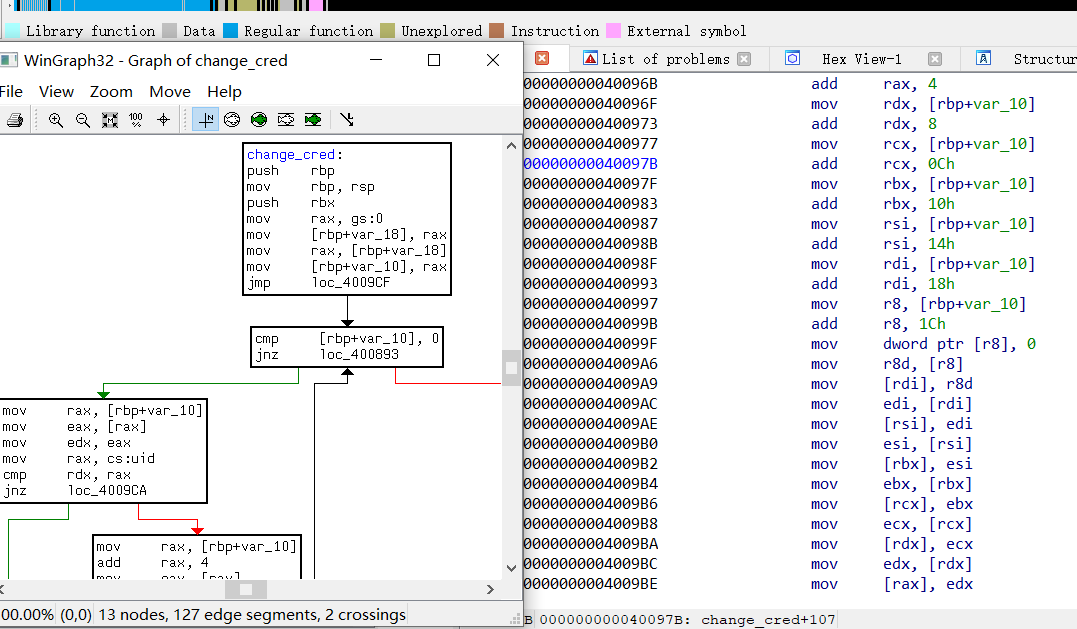
\includegraphics[width=0.75\textwidth]{figures/4.1}
	% \caption[这里的文字将会显示在 listoffigure 中]{这里的文字将会显示在正文中}
	\caption{IDA 反汇编 CFG 图}\label{fig:4.1}
\end{figure}


为确保扰动操作不影响原始程序逻辑,本文首先将反汇编得到的指令转换为一种自定义的中间表示(IR),该表示能记录每条指令的操作码、显式与隐式操作数、寄存器读写关系、以及影响到的标志位等静态语义信息。这种增强表示形式可有效辅助分析控制依赖与数据依赖关系,识别出可安全修改的指令区域。随后,本文实施三种语义保持的扰动技术:指令替换(Instruction Substitution)、指令重排序(Instruction Reordering) 和 寄存器重分配(Register Reallocation)。这三类方法分别从指令级别、顺序层级和寄存器使用层面引入扰动,旨在保持语义不变的前提下实现样本多样性和模型鲁棒性提升。

%To ensure disturbances do not disrupt the original program logic, the disassembled instructions are first transformed into a custom Intermediate Representation (IR). This IR records each instruction's static semantic information, such as opcode, explicit and implicit operands, register read and write relationships, and impacted flag bits, which effectively aids in analyzing control and data dependencies to identify safely modifiable instruction regions. Subsequently, three disturbance techniques—Instruction Substitution, Instruction Reordering, and Register Reallocation—ensure semantics are implemented. These methods respectively introduce disturbances at the instruction level, sequential layer, and register usage level, aiming to enhance sample diversity and model robustness while preserving semantics.

在变换过程中,所有修改操作均限制在已识别的、无控制依赖冲突的基本块内部,确保程序控制流图(CFG)保持稳定。如果某些变换操作(如指令顺序调整)导致代码地址偏移,本文会同步更新 ELF 文件中的相关重定位信息(如 .rela.text 段),以避免函数调用或跳转地址错误。整个扰动流程针对每个 ELF 文件独立执行,可自动生成多个等价但具有不同语法表现的扰动样本,用于训练或测试阶段的多样化增强,从而有效提升基于静态分析的恶意代码检测系统的鲁棒性。

%During transformation, all modifications are limited to identified basic blocks free of control dependency conflicts, ensuring Program Control Flow Graph (CFG) stability. If transformations like instruction resequencing cause code address shifts, relevant relocation information, such as .rela section and .text section, in the ELF file is synchronously updated to prevent faulty function call and jump address. This process executes per ELF file independently, automatically generating multiple syntactically distinct yet semantically equivalent adversarial samples. These enhance diversity in training and testing phases, effectively improving the robustness of malware detection systems based on static analysis.

(1) 指令替换(Instruction Substitution)

%(1) Instruction Substitution

指令替换作为一种二进制代码扰动方法,旨在通过将原始指令替换为等效的指令来扰乱程序的结构,同时保持程序的功能不变。该方法不仅能改变代码的外观,还能增加静态分析和逆向工程的难度。以下是指令替换的具体细节:

%Instruction substitution serves as a binary code disturbance method that alters program structure by replacing original instructions with equivalent ones while preserving program functionality. It not only disrupts code appearance but also increases the difficulty for static analysis and reverse engineering. Details are described as follows:
\begin{enumerate}

\item 等效指令替换:

%Equivalent Instruction Replacement:

在x86架构中,许多指令有多个等效形式,可以用不同的操作数或指令格式来实现相同的功能。例如:
add r/m32, r32 可以替换为 add r32, r/m32,这两者在操作数为寄存器时是等效的。

%On x86 architecture, many instructions have multiple equivalent forms, same functionality can be achieved by different operands and instruction forms.For example, “add r/m32, r32” can be replaced with “add r32, r/m32”, these two instructions are equivalent while operands are registers.

对于逻辑操作,test r/m8, r8 可以与 test r/m8, r/m8 等价。

%For logic operations, “test r/m8, r8” is equivalent to “test r/m8, r/m8”.

一些算术指令也有多个等效形式,比如 sub r/m32, r32 可以用 neg r/m32 替换(减法可以通过取负来实现)。

%Some arithmetic instructions also have multiple equivalent forms, such as “sub r/m32, r32” can be replaced with “neg r/m32”.

操作数形式替换指令时,可以改变操作数的形式,而不影响最终的计算结果。例如,mov r32, r/m32 和 mov r/m32, r32 都是等效的操作,但通过改变源和目标操作数的顺序,能够改变指令的字节表示。

%Operand forms can be altered when instructions are replaced, and do not affect ultimate calculation result. For example, “mov r32, r/m32” and “mov r/m32, r32” are equivalent operations, but the instruction byte expression can be altered by changing the sequence of source and target operands.

不同长度指令某些情况下,可以用长度相同但操作不同的指令替换原始指令,例如:
inc r32可以替换为 add r32, 1,二者功能相同,但指令长度和编码不同。

%In some circumstances, replacing original instructions with instructions that are the same length but different in operations are permitted.
%For example, “inc r32” can be replaced with “add r32, 1”, these two instructions have same functionality, different instruction length and coding.

dec r32可以替换为 sub r32, 1,实现同样的效果,增加了代码的复杂性。

%“dec r32” can be replaced with “sub r32, 1”, these two instructions have same effect, but increase code's complexity.

\item 替换控制流指令:

%Control Flow Instruction Replacement:

控制流指令(如跳转、条件跳转、调用等)也可以用等效的指令替换。例如:
jmp label 可以用 call label; pop 来替换,虽然实现了相同的跳转效果,但操作数和指令形式不同。

%Control flow instructions, such as jump, conditional jump, and call, can be replaced with equivalent instructions. For example, “jmp label” can be replaced with “call label; pop”, although two instructions achieve same jump result, but their operands and instruction forms are different.

je(等于跳转)可以替换为 jne(不等于跳转),并通过适当调整标志位来维持功能一致性。

%“je” can be replaced with “jne” by adjusting the flags properly to maintain functional consistency.

\item 确保指令长度一致:

%Maintain instruction length consistency:

由于对于许多stripped二进制文件,增加指令长度可能会导致代码结构破坏,因此在替换过程中要保证每条替换的指令与原指令长度相同。可以通过选择长度一致的等效指令来实现这一点,避免扰乱程序的整体布局。

%Increasing instruction length may cause code structure to be broken in many stripped binary files; thus, it is vital to ensure that each replaced instruction's length should be the same as the original. This can be achieved by selecting equivalent instructions that have the same length, avoiding disrupting the program's overall layout.

\item 随机化替换的应用方式:

%The application method of randomized replacement:

在替换指令时,可以根据一定的规则或随机选择等效指令来应用这些替换。替换不一定是对每条指令都应用,而是根据程序的特性和分析结果,选择性地对特定代码块进行替换。这种方法可以确保替换不会影响程序的控制流和逻辑结构,但同时会改变程序的外观,增加静态分析的难度。

%Replacements can be applied according to certain rules or randomized equivalent instruction selection. Replacements may not be applied to each instruction but are selectively applied to specific code blocks relying on program characteristics and analysis results. This method can ensure that replacements do not affect the program's control flow and logic structure but alter the program's appearance, increasing static analysis difficulty.

\end{enumerate}

通过以上方法,指令替换不仅保持程序功能的完整性,还有效增加了程序的混淆性,使得静态分析工具更难识别程序的真实意图,增加了逆向工程的复杂性。

%Through the methods above, instruction replacements not only maintain the program's complete functionalities but also increase the program's obfuscation, making it harder for static analysis tools to recognize the program's real intention and increasing the complexity of reverse engineering.

(2)指令重排序(Instruction Reordering)

%(2) Instruction Reordering
\begin{enumerate}


\item 基本块内部指令重排(Intra Basic Block Reordering):

%Intra Basic Block Reordering:

在一个基本块(Basic Block)中,若两条或多条指令之间没有数据或控制依赖关系,那么它们的执行顺序就是可以互换的。由于基本块是线性执行的中间代码区域,并且编译器在生成机器码时只是选择了若干等效顺序之一,因此只要保证依赖关系不变,修改指令顺序不会影响程序的功能。

%In a basic block, instructions without data and control dependencies can be reordered without affecting functionality. Since basic blocks are intermediate code areas for linear execution, and the compiler only selects one of equivalent sequences during machine code generation, thus instruction sequence modification does not affect the program's functionality if the dependency relationship remains unchanged.

本文对目标二进制程序进行反汇编,提取所有基本块。对每个基本块进行依赖分析,识别每条指令的读(use)和写(def)寄存器集。通过检测读后写(RAW)、写后读(WAR)、写后写(WAW)等依赖类型,构建出指令间的有向无环图(DAG)。

%This research disassembles target binaries to extract all basic blocks, then perform dependency analysis on each block, identifying each instruction's use and def register sets, constructing a Directed Acyclic Graph (DAG) among instructions by detecting RAW (Read-After-Write), WAR (Write-After-Read), and WAW (Write-After-Write) dependencies.

之后,使用拓扑排序枚举该图的合法指令顺序,并从中随机选取一种新的顺序,替代原始顺序。这一方法不会引入新的指令或修改指令操作数,因此保持程序的功能完全不变。它可以扰乱基于指令顺序或特征码的静态分析和检测机制,有效提升样本的多样性。

%Subsequently, this research enumerates legal instruction orders via topological sorting and randomly selects a new order to replace the original. This method can maintain the program's functionality because it does not introduce any new instructions or modify instruction operands. It disrupts static analysis mechanisms relying on instruction order or signatures, enhancing sample diversity.

\begin{figure}[hbt]
	\centering
	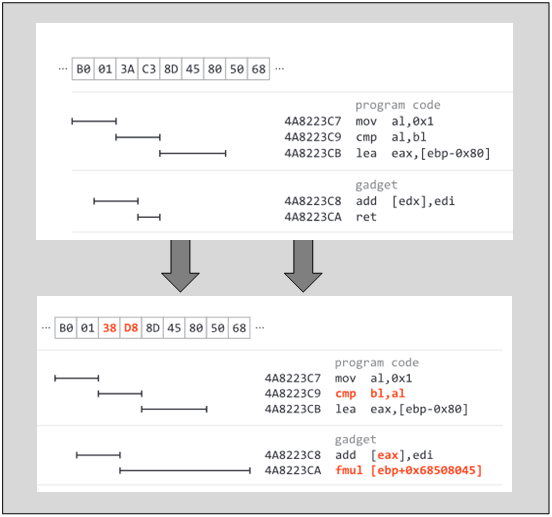
\includegraphics[width=0.75\textwidth]{figures/4.2}
	% \caption[这里的文字将会显示在 listoffigure 中]{这里的文字将会显示在正文中}
	\caption{指令替换示例图}\label{fig:4.2}
\end{figure}

\item 寄存器保护代码重排(Reordering of Register Preservation Code):

%Reordering of Register Preservation Code:

该方法基于函数调用时保存非易失性寄存器(callee-saved registers)所使用的push和pop指令的顺序是可变的,只要遵循“先进后出”的栈规则即可。即,函数在开头会使用若干push指令保存寄存器,函数结尾使用对应的pop恢复值。因为栈是倒序恢复的,所以只要保持pop顺序与push顺序相反,整个过程的语义就是等效的。

%This method is based on the theory that the sequence of push and pop instructions from callee-saved registers is alterable during function calls, which only need to follow the last-in-first-out (LIFO) stack rule. During function calls, the order of push (callee-saved registers) and corresponding pop instructions can vary if adhering to the last-in-first-out (LIFO) stack rule. Several push instructions are used by the function header to save data in registers, while corresponding pop instructions are used at the end of the function to restore values. Since the stack restores in reverse order, semantics during the entire process will be equivalent to the original if pop sequences are the opposite of push sequences.

%本文在函数的入口和出口识别出完整的寄存器保存/恢复代码段。对这些push和pop指令进行配对,确认其保护的是相同的寄存器,并追踪栈指针(ESP)的变化确保没有中间干扰。然后,对push序列进行重排,并将pop序列同步做相反的重排,确保恢复顺序正确。若push序列中夹杂有其他非保存性指令,也需进行依赖分析,保证重排不会打乱依赖顺序。这种方法对程序语义无影响,但能干扰基于特定pop序列模式的分析方法,提高静态分析、指令特征提取和样本分类的复杂度。

%This research identifies complete register save and restore code segments at the function entry and exit. Then pair push and pop instructions, ensuring that they operate on the same registers and track ESP changes to avoid other interference. Subsequently, reordering the push sequence and applying inverse reordering to pop sequence ensures restore proper sequence. If the push sequence contains other non-preservation instructions, dependency analysis is also essential to ensure that reordering does not disrupt dependency sequence. This method has no impact on the program's semantics but disturbs analysis methods based on specific pop sequence patterns, improving resistance to static analysis, instruction feature extraction, and classification.

\begin{figure}[hbt]
	\centering
	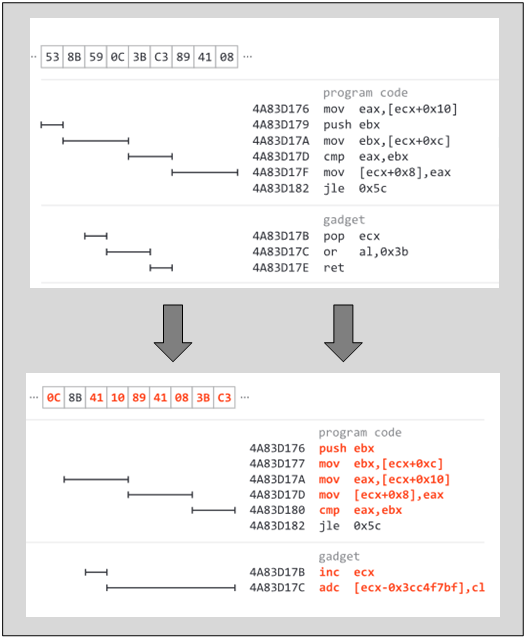
\includegraphics[width=0.75\textwidth]{figures/4.3}
	% \caption[这里的文字将会显示在 listoffigure 中]{这里的文字将会显示在正文中}
	\caption{指令重构排序示例图}\label{fig:4.3}
\end{figure}

\begin{figure}[hbt]
	\centering
	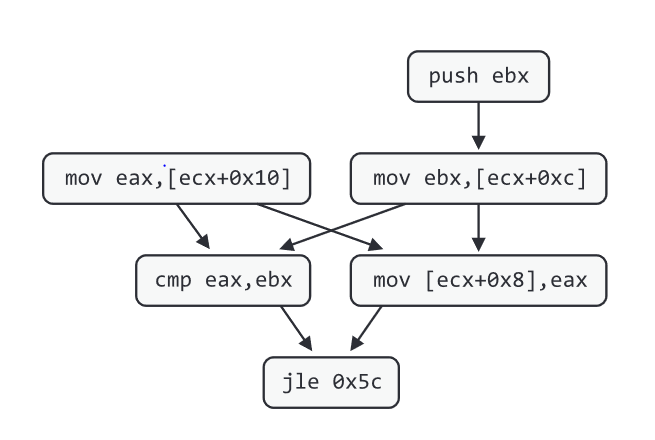
\includegraphics[width=0.75\textwidth]{figures/4.4}
	% \caption[这里的文字将会显示在 listoffigure 中]{这里的文字将会显示在正文中}
	\caption{重构的指令有序无环图}\label{fig:4.4}
\end{figure}

\begin{figure}[hbt]
	\centering
	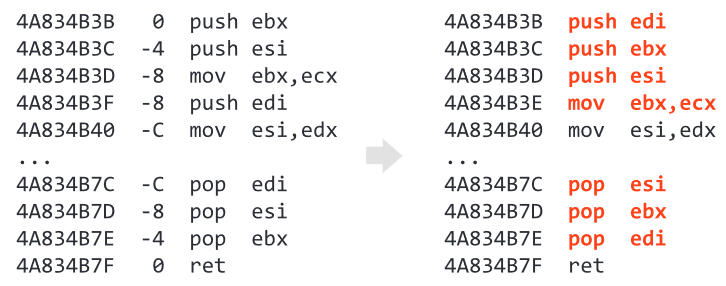
\includegraphics[width=0.75\textwidth]{figures/4.5}
	% \caption[这里的文字将会显示在 listoffigure 中]{这里的文字将会显示在正文中}
	\caption{寄存器保护代码重排序示例图}\label{fig:4.5}
\end{figure}

本文首先对二进制程序构建控制流图(CFG),并对每个基本块进行寄存器活跃性分析,获取每条指令的寄存器use(使用)与def(定义)集合。接着迭代计算每条指令的活跃输入集(in)与输出集(out),识别每个寄存器的活跃区域。在确保无冲突的前提下,随机选择两个不重叠活跃区的寄存器对,将其在汇编中的使用位置进行替换。指令修改时,通过变更ModR/M字节(必要时SIB字节)实现重映射,避免使用esp等特殊寄存器,并对隐式使用寄存器的指令进行过滤。为保证调用一致性,还需结合调用约定信息约束某些寄存器的使用。

%First, this method constructs the CFG for the binary program and performs register liveness analysis on each basic block to determine each instruction's register use and def sets. Second, this method iteratively computes each instruction's active in and out sets to identify live ranges in each register. On the premise that there is no conflict, two register pairs with non-overlapping live ranges are randomly selected, and then their usage positions are swapped in assembly. During instruction modification, modifying via ModR/M bytes (and SIB bytes if necessary) achieve remapping, avoiding special registers like ESP, filtering instructions with implicit register usage. To ensure call consistency, calling convention information is combined to constrain certain registers.

这一方法不会引入新指令或修改操作数值,仅在机器码层面更换寄存器编号,因此程序行为保持完全一致。该技术能有效打乱静态分析工具基于寄存器使用模式或特征序列的识别策略,从而提升样本的对抗性与多样性。

%This technique does not introduce any new instructions or change operand values, modifying only register encodings at the machine-code level. It disrupts static analysis tools based on register usage patterns or feature sequences recognition strategies, enhancing sample adversariality and diversity.
\end{enumerate}



\begin{figure}[hbt]
	\centering
	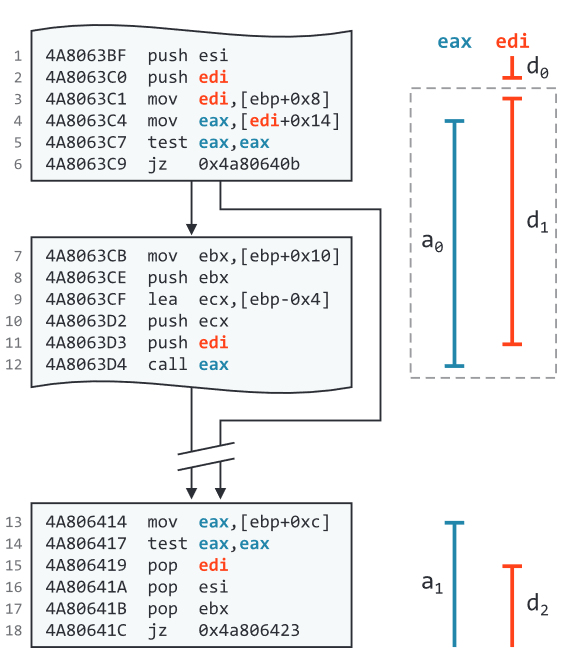
\includegraphics[width=0.75\textwidth]{figures/4.6}
	% \caption[这里的文字将会显示在 listoffigure 中]{这里的文字将会显示在正文中}
	\caption{寄存器重分配示例图}\label{fig:4.6}
\end{figure}

\subsection{动态行为扰动方法}

%在恶意软件检测领域,动态分析技术是当前主流手段之一,尤其在处理未知样本或多态变种时具有明显优势。其基本原理是通过在受控执行环境(如沙箱、虚拟机、内存监控器)中运行目标程序,记录其在运行过程中所触发的系统调用、行为路径、内存修改、网络通信等信息,以此识别潜在的恶意行为。然而,这一技术在实际部署中往往存在时间资源受限的问题。

为了兼顾效率与成本,动态分析系统通常仅为每个样本分配数秒到几十秒的执行时间窗口。对于某些攻击行为触发依赖于条件判断、用户交互的恶意样本而言,这一固定的分析时间窗显然存在被规避的可能性。

%In the malware detection realm, dynamic analysis technology is one of the currently prevalent approaches, demonstrating clear advantages when handling unknown or polymorphic variants. Its fundamental principle involves running target programs in controlled execution environments, such as sandboxes, virtual machines, and memory monitors, recording triggered system calls, behavioral paths, memory modifications, network communications, and other runtime information to identify potential malicious behaviors. However, this technology often faces time and resource constraints during deployment. To balance efficiency and cost, dynamic analysis systems commonly allocate only a few seconds to dozens of seconds of execution time to each sample. For malware whose attack behaviors depend on conditional triggers or user interaction, this fixed analysis window presents a probability of being evaded.

基于此观察,本文设计了一种动态扰动方法,核心思想是引入“时间延迟”机制,使恶意代码在样本启动后故意等待一段时间再执行核心逻辑,从而躲避沙箱的行为分析窗口。其主要实现方式是通过在程序入口点或关键路径中插入延迟逻辑(如 nanosleep系统调用),使恶意样本在运行初期不表现任何异常行为,从而骗过基于行为特征的检测系统。

%Based on this observation, this research designs a dynamic disturbance method whose central mechanism is introducing "time-delay", deliberately waiting for a period after startup before executing core logic, making the malicious code evade the behavioral analysis window of sandboxes. This is primarily implemented by inserting delay logic like the nanosleep system call at program entry points or critical paths, ensuring that the malware exhibits no abnormal behavior during the initial run phase and thus bypasses detection systems based on behavioral features.

具体而言,该方法在程序入口\_start 中插入一段系统调用延迟逻辑,构造一个 timespec结构体设置延迟时间(如60秒),并通过nanosleep系统调用实现挂起效果。在延迟期间,样本处于休眠状态,不触发任何系统调用,也不进行内存读写、网络通信等可疑操作。由于大多数沙箱系统会在执行时间到达后强制中止进程,此时还未触发的恶意行为链将完全无法被观测到。这样,恶意样本即使具有明显的破坏性,也可能因“未表现行为”而被误判为正常程序。

%Specifically, this method inserts system call delay logic at the \_start entry point. It constructs a timespec structure to set the delay duration and invokes the nanosleep system call to induce suspension. During this delay, the sample remains dormant, triggering no system calls, memory reads and writes, network communications, or other suspicious activities. As most sandbox systems forcibly terminate processes after exceeding the execution time limit, the un-triggered malicious behavioral chain remains entirely unobserved. Consequently, even obviously destructive malware may be misclassified as benign due to "absence of malicious behavior."

%该策略可归类为一种“动态行为隐藏技术”,其本质在于对行为时间的扰动,从时间维度上对抗行为检测系统。这类技术的优势在于实现成本低、兼容性好且对原有逻辑无破坏性,能够与其他扰动策略(如控制流平坦化、代码插桩、系统调用替换)联合使用,从而形成更强的检测对抗能力。

%This strategy can be classified as a "dynamic behavior concealment technique." Its essence is using timing disturbance behavior to counter detection systems temporally. Its advantages include low implementation cost, high compatibility, and non-destructive impact on original logic. It can also be combined with other disturbance strategies, such as control-flow flattening, code instrumentation, and system call replacement to form more robust evasion capabilities.

%值得注意的是,虽然该策略在现实场景中具有较强的隐蔽性,但其也可能被高级动态检测系统检测到。例如某些系统会使用加速执行技术(如时间跳跃模拟)、分析行为间歇性、或启用用户交互模拟等手段来破除延迟机制。因此,未来仍需结合其他对抗策略,共同提升样本的免杀能力和对抗鲁棒性。

%It is notable that this technique may still be detected by advanced dynamic analysis systems while having effective concealment in real scenarios. For example, some systems may employ execution acceleration techniques such as time-jump simulation, behavioral intermittency analysis, and user-interaction simulation, to counter delays. Therefore, future work should integrate other adversarial strategies to jointly enhance evasion and robustness.
\begin{algorithm}[htbp]
	\caption{使用可执行段填充空间进行 ELF 动态插入算法}
    \KwIn{目标 ELF 二进制文件路径 \texttt{input\_elf},载荷二进制代码路径 \texttt{code\_bin},输出 ELF 路径 \texttt{output\_elf}}
	\KwOut{一个已被感染的 ELF 文件,其中插入了载荷代码}
	Read the input ELF file \texttt{input\_elf} into memory \texttt{hdr}\;
	Read the payload binary code \texttt{code\_bin} into memory \texttt{code}\;
	Validate ELF magic number and ensure it is a 64-bit ELF\;
	Check if the ELF architecture is x86-64\;
	\ForEach{program header \texttt{phdr} in \texttt{hdr}}{
		\If{\texttt{phdr} is executable (has \texttt{PF\_X} flag)}{
			Find the last section \texttt{last\_sec} within \texttt{phdr}\;
			Compute the available padding size \texttt{pad\_size} after \texttt{last\_sec}\;
			\If{\texttt{pad\_size} $<$ size of \texttt{code} + size of jump}{
				Print error message and exit\;
			}
			Inject the payload \texttt{code} into the padding space\;
			Generate a jump instruction \texttt{jmp\_back} to the original entry point\;
			Inject \texttt{jmp\_back} after the \texttt{code}\;
			Modify the section header of \texttt{last\_sec} to extend its size\;
			Update the \texttt{phdr}'s file and memory size to include the injected code\;
			Update the ELF header's \texttt{e\_entry} to point to the start of the payload \texttt{code}\;
			\textbf{break}\;
		}
	}
	Write the modified ELF to \texttt{output\_elf}\;
	Set the file permission of \texttt{output\_elf} to executable\;
\end{algorithm}

基于时间延迟的动态扰动方法是一种有效的动态对抗技术,具有实现简单、效果明显、通用性强等优点,可作为恶意样本在强化学习训练与对抗生成中的关键扰动操作之一,具体实现如算法1所示。

%The disturbance method based on time delay is an effective dynamic adversarial technique that has advantages in simple implementation, high efficiency, and high versatility. It serves as a key disturbance operation for malware in reinforcement learning training and adversarial generation. Its concrete implementation is described in Algorithm 1 below.

算法1通过逐步操作,实现将载荷二进制代码动态插入到目标ELF可执行文件的可执行段填充空间中,保持原文件结构的同时实现控制流重定向。第1至2行将目标ELF文件与待插入的payload读入内存。第3至4行验证ELF文件的合法性,包括magic、是否为64位及是否为x86-64架构。第5至17行是注入的核心步骤:遍历每个程序头,第6行判断是否为可执行段(具有PF\_X标志),第7至8行定位该段的最后一个节并计算其后的空隙空间大小;若填充不足以插入payload与跳转指令,则退出(第9至10行)。第11至13行将载荷写入空隙并附加一段跳转回原始入口点的代码。随后,第14至15行扩展节和段的大小字段以覆盖新注入区域,确保在运行时被正确加载。第16行更新ELF头中的入口地址e\_entry为payload的起始位置,实现控制流重定向。完成注入后(第17行),退出循环以防止重复操作。最后,第18至19行将修改后的ELF写入输出文件并设置为可执行。整体流程在不破坏原有功能的前提下,实现了高隐蔽性和完整性兼容的动态插入操作。

%Algorithm 1 operates step-by-step, achieving inserting payload binary code into target ELF executable file's executable segment padding, maintaining original file structure while achieving control flow redirection. Lines 1 to 2 read target ELF file and payload into memory. Lines 3 to 4 check the legitimacy of ELF file, including magic number, whether it is 64 bits, and whether its architecture is x86-64. Lines 5 to 17 is the core process of injection, traversing each program header. Line 6 judges whether the segment is an executable segment that contains the PF\_X flag. Lines 7 to 8 locate the last section of this segment and calculate the gap size after it. Lines 9 to 10 terminate the process when the gap size cannot accommodate the payload and jump instructions. Lines 11 to 13 write the payload to the gap and append code block that jumps to the original entry point. Subsequently, lines 14 to 15 expand the size fields of the section and segment to cover newly injected areas to ensure that it can be loaded correctly during execution. Line 16 updates the entry point e\_entry in the ELF header to be the starting point of payload, achieving control flow redirection. Line 17 exits the loop to prevent duplicate operations after the injection is completed. Finally, lines 18 to 19 write the modified ELF file to an output file and set it as an executable file. The overall process achieves dynamic insertion operations that exhibit high concealment and complete compatibility in the condition that the original functionality is not broken.

\section{奖励函数策略优化}

%(3) Reward Function Strategy Optimization

在本研究中,强化学习(RL)模型的奖励函数设计是生成对抗性恶意软件样本的核心要素之一。为了使智能体能够有效地避开恶意软件检测系统,并生成具有足够复杂性的对抗样本,本文提出了一种综合考虑检测逃逸、样本多样性和生成复杂度的奖励函数。奖励函数的优化与构建直接决定了智能体在训练过程中的学习效果和最终生成的恶意样本的质量。

%In this research, designing the reward function for the RL model is a core element for generating adversarial malware samples. To enable the agent to effectively evade malware detection systems and generate adversarial samples with sufficient complexity, this research proposes a reward function that comprehensively considers evasion success, sample diversity, and generation complexity. The optimization and construction of the reward function directly determine the agent's learning effectiveness during training and final generated malicious samples' quality.

首先,奖励函数的主要目标是鼓励智能体生成能够避开现有检测系统的恶意样本。因此,奖励函数首先根据样本是否能够逃避检测来给予奖励。当智能体生成的样本未被恶意软件检测模型判定为恶意时,智能体将获得一个正向奖励,反之则给予负向奖励。这个反馈机制可以引导智能体在生成过程中不断优化策略,以提高恶意样本的逃逸能力。

%First, the primary goal of the reward function is to encourage the agent to generate malicious samples that can evade existing detection systems. Therefore, the reward function grants rewards based on whether the sample successfully evades detection. When the sample generated by the agent is not classified as malicious by the malware detection model, the agent receives a positive reward; otherwise, it receives a negative reward. This feedback mechanism guides the agent to continuously optimize its strategy during generation, thereby improving the evasion capability of malicious samples.

其次,样本的多样性也是奖励函数中一个重要的考虑因素。在对抗性样本生成过程中,若智能体能够通过修改程序的控制流、修改函数调用顺序、插入随机字符串等方式增加样本的多样性,将会获得相应的奖励。通过这种方式,奖励函数促进了恶意样本的多样化,避免了模型生成过于单一或重复的样本,从而提高了生成样本的泛化能力。

%Second, sample diversity is also a critical factor that should be considered in the reward function. During adversarial sample generation process, if the agent increases sample diversity by modifying control flow, altering function call sequences, or inserting random strings, it receives corresponding rewards. This approach promotes the diversification of malicious samples, avoids generating monotonous or duplicate samples, and enhances the generalization ability of generated samples.

最后,为了避免智能体在生成样本时产生过于复杂或不稳定的结果,本文在奖励函数中引入了对样本复杂度的惩罚机制。当生成的恶意样本过于复杂(例如,通过过多的控制流操作或冗长的代码片段),智能体将受到一定的惩罚。这一策略帮助智能体在保证逃逸能力的同时,生成更加稳定和有效的样本,从而提高生成的样本的实际应用价值。

%Finally, to prevent the agent from generating overly complex or unstable results, the reward function incorporates a penalty mechanism for sample complexity. If a generated malicious sample is excessively complex, such as containing too many control flow operations or lengthy code fragments, the agent is penalized. This strategy helps the agent generate more stable and effective samples while ensuring evasion capability and enhancing the practical application value of generated samples.

%为了使奖励函数更加灵活和适应不同训练阶段,本文还采用了动态调整策略。在训练的初期,智能体主要依赖于探索奖励,通过多样化的变异操作来探索不同的恶意样本类型。随着训练的进展,探索奖励逐步减少,智能体将更多地依赖于利用已知的优秀策略,以生成更加高效和复杂的恶意样本。这种动态调整机制确保了智能体能够在探索和利用之间找到平衡,并逐步提升生成样本的质量。

%To make the reward function more flexible and adaptable to different training phases, this research adopts a dynamic adjustment strategy. In the initial training phase, the agent primarily relies on exploration rewards to explore diverse mutation operations and generate various malicious sample types. As training progresses, exploration rewards gradually decrease, and the agent increasingly relies on known effective strategies to generate more efficient and complex malicious samples. This dynamic adjustment ensures that the agent finds a balance between exploration and exploitation, progressively improving the quality of generated samples.

传统对抗样本生成方法多采用固定或静态的奖励函数,往往仅考虑单一的检测规避结果,例如是否成功逃避分类器或沙箱分析系统\cite{anderson2018learning}。然而,在实际应用场景中,恶意样本的行为表征、检测机制、资源限制(如沙箱分析时长)等因素均具备高度动态性。因此,本文设计一种自适应、阶段感知和行为敏感的动态奖励函数策略,对于提升对抗样本生成质量和鲁棒性具有重要意义。

%Traditional adversarial sample generation methods mostly adopt fixed or static reward functions, often considering only a single evasion detection result, such as whether the sample successfully evades a classifier or a sandbox analysis system\cite{anderson2018learning}. However, in real application scenarios, factors such as malware behavioral characteristics, detection mechanisms, and resource constraints, such as sandbox analysis duration, exhibit high dynamism. Therefore, this research designs an adaptive, stage-aware, and behaviorally sensitive dynamic reward function strategy that is significant for improving the quality and robustness of adversarial sample generation.

\subsection{奖励函数设计动机}

强化学习智能体的行为策略直接受其奖励信号驱动。若奖励仅依据“是否逃避成功”这一单一信号,则智能体可能在初始训练阶段陷入稀疏奖励困境,导致训练效率低下,策略不稳定,甚至难以收敛。为解决该问题,本方法引入多源奖励信号融合机制,综合以下三类指标:

%The behavioral policy of a reinforcement learning agent is directly driven by its reward signals. If rewards are solely based on the singular signal of "whether evasion is successful," the agent may face sparse reward dilemmas during initial training phases, resulting in inefficient training, unstable strategies, or even failure to converge. To address this issue, this research proposes a method that introduces a multi-source reward signal fusion mechanism, integrating the following three metrics:
\begin{enumerate}
\item 规避性得分(Evasion Score):反映样本是否成功规避沙箱或机器学习检测模型,是核心奖励来源;

%Evasion Score: It reflects whether the sample successfully evades sandbox or machine learning detection models, serving as the primary reward source.

\item 扰动成本(Perturbation Cost):衡量修改对原始样本的干扰程度,用于抑制过度修改,保持样本可执行性与语义一致性;

%Perturbation Cost: It measures the perturbation degree of modifications to the original sample, suppressing excessive alterations to maintain executability and semantic consistency.

\item 行为混淆度(Behavior Confusion Degree):衡量样本行为与正常软件的相似度,鼓励智能体生成更具隐蔽性的扰动策略。

%Behavior Confusion Degree: It measures the similarity between sample behavior and benign software, encouraging the agent to generate more stealthy disturbance strategies.
\end{enumerate}

\subsection{奖励函数表达形式}
 
定义智能体在时刻 $t$ 执行扰动动作 $a_t$ 后的奖励 $R_t$ 为多项加权组合:

%The reward $R_t$ for the agent after executing disturbance action $a_t$ at time $t$ is defined as a weighted combination:
\begin{equation}
	R_t = \lambda_1 \cdot R_{\text{evasion}} + \lambda_2 \cdot R_{\text{confusion}} - \lambda_3 \cdot R_{\text{cost}}
\end{equation}

其中,$R_{\text{evasion}}$ 表示若样本成功绕过沙箱或分类器则给予正奖励,否则为 0;$R_{\text{confusion}}$ 表示根据行为序列(如系统调用图)与良性样本的相似度计算得分,例如使用 Jaccard 相似度或结构相似性;$R_{\text{cost}}$ 表示扰动的代价,可以根据扰动次数、修改字节数以及修改位置的敏感度等进行计算;$\lambda_1$、$\lambda_2$ 和 $\lambda_3$ 为动态可调的权重参数。

%In this formulation, $R_{\text{evasion}}$ represents that if the sample evade the sandbox or classifier, positive reward should be given, otherwise, the reward is zero; $R_{\text{confusion}}$ represents a score calculated from the similarity between behavioral sequence, such as system call graphs, and benign samples, such as using Jaccard similarity or structural similarity; $R_{\text{cost}}$ denotes the disturbance cost that is calculated based on number of disturbances, modified bytes, and sensitivity of modified locations; $\lambda_1$, $\lambda_2$, and $\lambda_3$ are dynamically adjustable weighting parameters.
\section{强化学习模型构建与训练}

%(4) Reinforcement Learning Model Construction and Training

%在前述模型架构中,本文设计了强化学习的智能体,旨在通过持续优化恶意软件样本生成过程以规避检测。为了提升智能体的决策能力和生成样本的多样性,本文采用了LSTM和PPO相结合的强化学习模型。

%In the model structure proposed previously, this research designs a RL agent aimed at continuously optimizing the malware sample generation process to evade detection. To enhance the agent's decision-making capability and the diversity of generated samples, this research adopts an RL model combining LSTM and PPO.

%首先,LSTM被集成到智能体的策略网络中,以便捕捉生成过程中的长期依赖关系。恶意软件样本的生成过程通常是序列化的,每一步生成的行为不仅依赖于当前的输入,还受到之前生成步骤的影响。LSTM作为一种循环神经网络,能够有效存储并利用这些历史信息,从而增强模型在生成恶意样本时的准确性和灵活性。通过这种方式,智能体能够在执行每一个生成操作时考虑到先前的生成状态,进而做出更加合理的决策,减少生成结果的不一致性。

%First, LSTM is integrated into the agent's policy network to capture long-term dependencies in the generation process. Malware sample generation is commonly sequential. Each generation step depends not only on the current input but also on prior steps. As a recurrent neural network, LSTM effectively stores and utilizes historical information, enhancing the accuracy and flexibility of the model during malware generation. This solution enables the agent to consider previous generation states when performing each operation, make more reasonable decisions and reduce inconsistencies in generated results.

%在此基础上,PPO强化学习算法被用来进一步优化策略的更新过程。PPO作为一种近端策略优化方法,利用了较为稳定的策略更新机制,有效避免了策略的剧烈波动。通过控制每次策略更新的幅度,PPO能够保证智能体在不断尝试和学习的过程中,既能够快速提高生成效果,又能避免由于过度优化而导致的不稳定。PPO通过对策略网络的不断优化,使得智能体能够逐步学会如何在恶意软件生成过程中最大化逃避检测系统的概率,从而提高生成样本的攻击性和隐蔽性。

%On this basis, the PPO RL algorithm is used to optimize the policy update process further. As a proximal policy optimization method, PPO adopts a stable update mechanism, effectively avoiding severe policy fluctuations. By controlling the magnitude of each policy update, PPO ensures the agent rapidly improves generation performance while preventing the model from being unstable due to over-optimization. Through PPO continuously optimizing the policy network, the agent can progressively learn how to maximize evasion probability against detection systems during malware generation, thereby enhancing the aggressiveness and concealment of generated samples.

%在训练过程中,智能体每生成一个恶意软件样本,就会根据检测模型给出的评分作为奖励反馈给智能体。这些奖励信号作为训练的动力,推动策略网络的优化。为了增强训练的稳定性,本文采用了经验回放机制和奖励归一化技术。这些方法使得智能体在学习过程中能够更加高效地利用过去的经验,同时避免由于奖励过大或过小导致学习不平衡的情况。

%During the training process, each time the agent generates a malware sample, the detection model's evaluation is provided as feedback to the agent. These rewards serve as training incentives to promote strategy network optimization. To enhance training stability, this research employs an experience replay mechanism and reward normalization techniques that enable the agent to utilize past experiences more efficiently and prevent learning imbalance from excessively large or small rewards.

%通过这种结合LSTM和PPO的方法,智能体能够在恶意软件生成任务中不断优化其生成策略。最终,训练完成的模型能够生成具有高度复杂性和隐蔽性的恶意软件样本,这些样本能够有效地避开现有的恶意软件检测系统,提升了对抗性样本生成的能力。

%Through this method combining LSTM and PPO, the agent continuously optimizes its generation strategies for malware generation tasks. Ultimately, the trained model can generate highly complex and stealthy malware samples that effectively evade current malware detection systems, significantly advancing adversarial sample generation capabilities.

本章提出的基于PPO(Proximal Policy Optimization)与 LSTM(Long Short-Term Memory)结合的强化学习模型主要由四个部分组成:LSTM时间特征编码层、策略网络(Actor)、价值网络(Critic)以及PPO优化器。训练过程中,首先由策略网络根据当前环境状态生成动作概率分布,同时价值网络对当前状态进行价值评估。为了能够有效建模动作序列中的时间依赖性,引入了LSTM模块,使得模型能够记忆过去的历史状态信息,捕获长期依赖特征,从而提升策略的稳定性与鲁棒性。最后,通过PPO优化器对策略进行迭代更新,保证训练过程中策略更新的稳定性与高效性。

%The reinforcement learning model combining PPO and LSTM, proposed in this chapter, consists of four main components: an LSTM temporal feature encoding layer, a policy network (Actor), a value network (Critic), and a PPO optimizer. During the training process, first, the policy network generates an action probability distribution based on the current environment state. Concurrently, the value network evaluates the value of the current state. To effectively model temporal dependencies in action sequences, the LSTM module is introduced, which enables the model to record historical state information and capture long-term dependency features, enhancing policy stability and robustness. Finally, the PPO optimizer iteratively updates the policy, ensuring stable and efficient policy updates throughout the training process.

\begin{algorithm}[htbp]
	\caption{基于强化学习的 ELF 对抗样本生成算法}
	\KwIn{原始 ELF 恶意样本集 $S$,最大迭代次数 $I$,预训练模型 $M$(PPO+LSTM),免杀行为表 \texttt{Action\_table},检测结果记录表 \texttt{Re}}
	\KwOut{免杀后的样本集 $S$}
	初始化智能体 agent 与环境 env\;
	agent $\leftarrow$ PPO\_LSTM.load($M$)\;
	$R_d \leftarrow 0$\;
	\ForEach{$s \in S$}{
		env.reset()\;
		tag $\leftarrow$ env.detect($s$)\;
		$S_t \leftarrow [\ ]$\;
		\For{$i \leftarrow 1$ \KwTo $9$}{
			$S_t \leftarrow S_t + \texttt{env.extractor}(s, i)$\;
		}
		\For{$j \leftarrow 1$ \KwTo $I$}{
			act $\leftarrow$ agent.predict($S_t$, $R_d$)\;
			\If{tag == benign}{
				\textbf{break}\;
			}
			$s \leftarrow \texttt{env.step}(s, \texttt{Action\_table}[act])$\;
			$S_t \leftarrow [\ ]$\;
			\For{$i \leftarrow 1$ \KwTo $9$}{
				$S_t \leftarrow S_t + \texttt{env.extractor}(s, i)$\;
			}
			tag $\leftarrow$ env.detect($s$)\;
			
			计算规避性得分:\texttt{Evasion\_Score} $\leftarrow$ score\_function($s$)\;
			
			计算行为混淆度:\texttt{Behavior\_Confusion\_Degree} $\leftarrow$ calculate\_confusion\_degree($s$)\;
			
			计算扰动成本:\texttt{Perturbation\_Cost} $\leftarrow$ calculate\_perturbation\_cost($s$, \texttt{Action\_table}[act])\;
			
			\If{tag == benign}{
				$R_d \leftarrow 10 \cdot \texttt{coefficient1} + \texttt{Behavior\_Confusion\_Degree} - \texttt{Perturbation\_Cost}$\;
				\textbf{break}\;
			}
			\Else{
				$R_d \leftarrow \texttt{Behavior\_Confusion\_Degree} - \texttt{Perturbation\_Cost}$\;
			}
		}
		\texttt{Re[$s$]} $\leftarrow$ tag\;
	}
\end{algorithm}

算法2描述了通过强化学习(PPO+LSTM)模型生成ELF格式恶意样本的免杀对抗样本。第1至2行初始化智能体和环境,加载预训练的PPO+LSTM模型。第3行初始化奖励信号$R_d$为0。第4至6行遍历原始恶意样本集$S$并重置环境,检测样本的标签。第7至9行提取环境中的特征,并存储在状态$S_t$中。第10至26行是主要的扰动步骤:智能体根据当前状态和奖励预测执行动作。第11至12行通过智能体的预测生成扰动动作,并根据样本标签(恶意或良性)决定是否继续执行。第13至15行,执行动作后更新样本并提取新的环境特征。第16至18行,计算新的奖励值,综合考虑规避性得分、行为混淆度和扰动成本。第19至24行根据检测结果和扰动成本动态计算奖励值,如果样本成功规避检测则给予较高的奖励,否则计算扰动成本并适当降低奖励。第27行更新样本的标签并记录在检测结果表Re中。整个流程通过多源奖励信号的融合与动态调整,逐步优化智能体的策略,以生成能够有效绕过检测并保持样本可执行性的对抗样本。

%Algorithm 2 describes the ELF-format malware adversarial sample generation process that uses a reinforcement learning model based on PPO and LSTM. Lines 1 to 2 initialize the agent and environment, loading the pre-trained PPO+LSTM model. Line 3 initializes the reward signal $R_d$ to 0. Lines 4 to 6 iterate through the original malicious sample set $S$, reset the environment, and detect the sample's label. Lines 7 to 9 extract features from the environment and store them in state $S_t$. Lines 10 to 26 are the core disturbance steps: the agent predicts an action based on the current state and reward signal. Lines 11 to 12 generate disturbance actions based on the agent's prediction and decide whether to continue according to whether the sample's label is benign or malicious. After executing actions, lines 13 to 15 update samples and extract novel environmental characteristics. Line 16 to 18 calculate novel reward value comprehensively based on evasion score, behavior confusion degree, and disturbance cost. Line 19 to 24 dynamically calculates reward values according to the detection result and disturbance cost. If the sample evades detection successfully, higher rewards will be granted. Otherwise, the disturbance cost is calculated, and rewards are penalized. Line 27 updates the sample's label and records it in the result table Re. The whole process gradually optimizes the agent's strategies through merging multi-source signals and adjusting dynamically, generating adversarial samples that evade detection effectively while maintaining executability.

\subsection{LSTM时间特征编码层}

在传统强化学习中,策略与价值估计往往只基于当前状态单步决策,忽略了历史决策之间的时间关联性,容易导致短视行为。

%In traditional RL, policy and value estimation usually rely solely on single-step decisions based on the current state, neglecting temporal correlations among historical decisions. This can lead to short-sighted behavior.

为此,本模型在输入端引入了LSTM(长短期记忆网络),通过门控机制捕获长期依赖,增强决策的时序连贯性。

%To address this issue, the model introduces an LSTM layer at the input stage. Through gating mechanisms, LSTM captures long-term dependencies, enhancing the temporal coherence of decision-making.

LSTM单元内部操作公式如下:

%Internal operation formulations of the LSTM unit are defined as follows:

输入门(控制当前输入信息的流入):

%Input Gate (controlling the flow of current input information):
\begin{equation}
i_t = \sigma(W_i x_t + U_i h_{t-1} + b_i)
\end{equation}

遗忘门(控制上一个记忆单元的保留程度):

%Forget Gate (controlling retention level of the previous memory cell):
\begin{equation}
f_t = \sigma(W_f x_t + U_f h_{t-1} + b_f)
\end{equation}

单元状态更新(生成新的记忆内容):

%Cell State Update (Generating new memory content):
\begin{equation}
\tilde{c}_t = \tanh(W_c x_t + U_c h_{t-1} + b_c)
\end{equation}

单元状态(记忆细胞)更新:

%Cell State Update (memory cell):
\begin{equation}
c_t = f_t \odot c_{t-1} + i_t \odot \tilde{c}_t
\end{equation}

输出门(控制隐藏状态输出):

%Output Gate (controlling hidden state output):
\begin{equation}
o_t = \sigma(W_o x_t + U_o h_{t-1} + b_o)
\end{equation}

隐藏状态更新(作为下一步输出):

%Hidden State Update (output for the next step):
\begin{equation}
h_t = o_t \odot \tanh(c_t)
\end{equation}

其中,$\sigma$ 为 Sigmoid 激活函数,$\odot$ 表示 Hadamard 乘积(元素乘),
$x_t$ 是当前时刻的输入状态,$h_{t-1}$ 和 $c_{t-1}$ 分别是上一时刻的隐藏状态与单元状态。

%In the formulations, $\sigma$ is the Sigmoid activation function. $\odot$ represents the Hadamard product in element multiplication. $x_t$ is the input state of current time. $h_{t-1}$ and $c_{t-1}$ are the hidden state and cell state of the previous time step.

通过以上机制,LSTM 能有效捕捉输入状态序列中的长期依赖特征,使策略网络与价值网络
具有更强的历史建模能力。

\subsection{策略网络(Actor)}

策略网络负责从环境中接收到的状态信息中,输出当前动作的概率分布。为了增强策略对于历史信息的感知能力,策略网络在输入端接入了LSTM层,LSTM能够在一定程度上记忆先前状态的隐藏信息,从而使得输出的策略不仅依赖当前时刻的观测,还综合考虑了历史观测序列的特征。
策略网络的目标是根据当前的隐藏状态$h_{t}$,输出每个动作的概率分布$\pi_{\theta}(a_{t}|s_{t})$ 。
具体过程如下:

%The policy network receives environmental state information and outputs the probability distribution of current actions. To enhance its awareness of historical information, the policy network introduces an LSTM layer at the input stage. The LSTM records hidden information from previous states, enabling the output policy to rely on not only the current observation but also features from historical observation sequences. The policy network's goal is to output each action's probability distribution $\pi_{\theta}(a_{t}|s_{t})$ based on the current hidden state $h_{t}$. The concrete processes are listed below:

\begin{enumerate} [label=\arabic*)] 

\item LSTM编码后的隐藏状态$h_{t}$作为输入;

%The LSTM-encoded hidden state $h_{t}$ serves as input.

\item 经过多层感知机(MLP)映射至动作空间;

%A multilayer perceptron (MLP) maps this to the action space.

\item 通过 Softmax 函数输出动作分布:

%The Softmax function outputs the action distribution:
\begin{equation}
\pi_{\theta}(a_t | s_t) = Softmax(W_p h_t + b_p)
\tag{4.8}
\end{equation}
其中,$W_p$、$b_p$ 为策略网络的权重与偏置参数,$\theta$ 表示策略网络的参数集合;

%In this formulation, $W_p$ and $b_p$ are the policy network's weight and bias parameters, and $\theta$ represents the policy network's parameter set.

\item 依据动作概率分布进行采样,生成动作 $a_t$:

%Actions $a_t$ are generated according to the sampling from the probability distribution.
\begin{equation}
a_t \sim \pi_\theta(a_t | s_t)
\end{equation}

\end{enumerate}
%This mechanism enables the LSTM to effectively capture long-term dependencies in input state sequences, enhancing the historical modeling capability of the policy and value networks.

%\section{本章小结 Chapter Summary}

%本章首先介绍了当前恶意软件检测领域中面临的挑战,特别是在应对新型对抗性样本时,传统的检测方法往往无法有效识别。通过分析现有技术的不足之处,发现许多传统方法所存在的问题。针对这些问题,本章提出了对应的解决方案。接下来,本章详细介绍了这一解决方案的设计思路。通过强化学习算法,代理能够在训练环境中与检测模型互动,学习如何生成绕过检测的恶意样本。这一过程通过奖励机制引导代理生成具有高隐蔽性和变异性的样本,从而提升恶意软件的复杂度和变化性,使得现有的检测方法更难识别。最后,本章描述了整个系统的整体架构设计。该架构包括数据收集与处理、扰动策略构建、奖励函数策略优化与强化学习模型构建与训练四个部分以实现本文的研究目标,完成对抗样本的生成。

%First, this chapter introduces the challenges faced in the malware detection realm, particularly the severe condition that traditional malware detection methods are ineffective at detecting novel adversarial samples. Through an analysis of existing techniques, many shortcomings existing in traditional methods are pointed out. To address current technology issues, this chapter presents corresponding solutions. It then provides detailed design logic for these solutions. By adopting reinforcement learning algorithms, the agent interacts with detection models in a training environment to learn how to generate malicious samples that can evade detection. This process is guided by reward mechanisms that encourage the agent to generate highly stealthy and variable samples to enhance malware complexity and variability, making it harder for existing detection methods to identify them. Finally, the chapter describes the overall system architecture that comprises four key components: data collection and processing, disturbance strategy construction, reward function strategy optimization, and RL model construction and training. This architecture is designed to achieve the research target, successfully generating adversarial samples.